\documentclass[11pt]{article}
\usepackage[parfill]{parskip}
\usepackage{graphicx}
\usepackage{wrapfig}
\usepackage{subcaption}
\usepackage[top=1in, bottom=1in, left=1in, right=1in]{geometry}
\bibliographystyle{plain}
\usepackage{amsmath}
\usepackage{amsfonts}
\usepackage{hyperref}
\usepackage{listings}
\usepackage{xcolor}
%%%%%%%%%%%%%%%%%%%%%%%%%%%%%%%%%%%%%%%%%%%%%%%%%%%%%%%%%%%%%%%
\usepackage{fancyhdr}
\pagestyle{fancy}
%%% Please add the author's last names
\lhead{Galois TA2 AMIDOL}
\rhead{ASKE Phase 1 Report}
%%% Please use \cfoot{} to remove page numbers
\cfoot{ }
\renewcommand{\headrulewidth}{0pt}
\renewcommand{\footrulewidth}{0pt}
%%%%%%%%%%%%%%%%%%%%%%%%%%%%%%%%%%%%%%%%%%%%%%%%%%%%%%%%%%%%%%&
\usepackage{titlesec}
\titlespacing{\section}{0pt}{\parskip}{-.5\parskip}
\titlespacing{\subsection}{0pt}{\parskip}{- .5\parskip}
\titlespacing{\subsubsection}{0pt}{\parskip}{- .5\parskip}
\newcommand{\closeup}{\setlength{\itemsep}{-4pt}}

\colorlet{punct}{red!60!black}
\definecolor{background}{HTML}{EEEEEE}
\definecolor{delim}{RGB}{20,105,176}
\colorlet{numb}{magenta!60!black}

\lstdefinelanguage{json}{
    basicstyle=\normalfont\ttfamily,
    numbers=left,
    numberstyle=\scriptsize,
    stepnumber=1,
    numbersep=8pt,
    showstringspaces=false,
    breaklines=true,
    frame=lines,
    backgroundcolor=\color{background},
    literate=
     *{0}{{{\color{numb}0}}}{1}
      {1}{{{\color{numb}1}}}{1}
      {2}{{{\color{numb}2}}}{1}
      {3}{{{\color{numb}3}}}{1}
      {4}{{{\color{numb}4}}}{1}
      {5}{{{\color{numb}5}}}{1}
      {6}{{{\color{numb}6}}}{1}
      {7}{{{\color{numb}7}}}{1}
      {8}{{{\color{numb}8}}}{1}
      {9}{{{\color{numb}9}}}{1}
      {:}{{{\color{punct}{:}}}}{1}
      {,}{{{\color{punct}{,}}}}{1}
      {\{}{{{\color{delim}{\{}}}}{1}
      {\}}{{{\color{delim}{\}}}}}{1}
      {[}{{{\color{delim}{[}}}}{1}
      {]}{{{\color{delim}{]}}}}{1},
}

\newcommand{\amidol}{\textsc{AMIDOL}}

\def\signed #1{{\leavevmode\unskip\nobreak\hfil\penalty50\hskip2em
  \hbox{}\nobreak\hfil(#1)%
  \parfillskip=0pt \finalhyphendemerits=0 \endgraf}}

\newsavebox\mybox
\newenvironment{aquote}[1]
  {\savebox\mybox{#1}\begin{quote}}
  {\signed{\usebox\mybox}\end{quote}}

\date{\vspace{-5ex}}
% Use this to get rid of the date

\usepackage{authblk}
\author[1]{Eric Davis}
\author[1]{Alec Theriault}
%\author[1]{Max Orhai}
%\author[1]{Eddy Westbrook}
\author[1]{Ryan Wright}
\affil[1]{Galois, Inc}

%\setcounter{page}{0}



\title{ASKE Phase 1 Report for \amidol{}}

\begin{document}
\maketitle
\vspace{10pt}

\section{Introduction}

Phase 1 of the \amidol{} project for ASKE has focused on proving out the initial concepts, theories, algorithms, and defining the core architectures, domain specific languages, and intermediate representations necessary to support the ambitious goal of advancing the state of the art of complex system analysis and machine-assisted science in ways that lower the overhead requirements in terms of large teams of domain experts, data scientists, mathematicians, and software engineers.  \amidol{}: the Agile Metamodel Interface using Domain-specific Ontological Languages, aims to reduce the overhead associated with the model life cycle and to enable domain experts and scientists to more easily build, maintain, and reason over models in robust and highly performable ways, and to respond rapidly to emerging crises in an agile and impactful way.  We do this by addressing the lack of generalizability, poor performance, and difficulties encountered when attempting to synthesize actionable knowledge and policies from the raw outputs of mathematical models.

\amidol{} is designed to support models in a number of scientific, physical, social, and hybrid domains by allowing domain experts to construct meta-models in a novel way, using visual domain specific ontological languages (VDSOLs).  These VDSOLs utilize an underlying intermediate abstract representation to give formal meaning to the intuitive process diagrams scientists and domain experts normally create.  \amidol{} then provides translations from these VDSOLs into an intermediate representation which can be transformed as appropriate to compose models, apply optimizations, and translate them into executable representations allowing \amidol{}'s inference engine to execute prognostic queries on reward models and communicate results to domain experts. In Phase 2\amidol{} will bind these results to the original ontologies providing more explainability when compared to conventional methods.

\amidol{} addresses the problem of machine-assisted inference with two high-level goals:

\begin{enumerate}
\item improving the ability of domain experts to build and maintain models and
\item improving the explainability and agility of the results of machine-inference.
\end{enumerate}

The VDSOLs help achieve these goals by lowering the barrier for entry associated with formal modeling languages.  VDSOLs allow the expression of rich mathematical concepts using visual diagrams for systems and processes.  The \amidol{} intermediate representation backs these diagrams with mathematical meaning, and allows the creation of new VDSOL elements as necessary with full expressivity, and Turing completeness.  The use of the intermediate representation also allows \amidol{} to decouple the problem of model optimization, performance, and implementation from the task of model definition, ensuring any model defined in any VDSOL is translated to the same abstract representation.  This abstraction can then be transformed using a set of well defined operations, eventually resulting in executable code which the \amidol{} inference engine can execute.  Because \amidol{} uses a universal representation for this intermediate form, models defined with \amidol{} can be easily ported to off the shelf solution techniques which have already been vetted by the community, and optimized for high performance computing.

The Phase 1 Prototype for \amidol{} shows a proof of concept of the core capabilities required to achieve this full vision in Phase 2, and has helped to identify the necessary next steps in realizing a the full framework as part of the ASKE program.  We include in our prototype three VDSOLs to show flexibility, and two backend targets already in use by the community.

\section{\amidol{} Architecture}

\amidol{}'s architecture is illustrated in Figure \ref{Fig:AMIDOLArch}.  It consists of three main components, the UI Editor which allows for the definition of models in an appropriate VDSOL, the \amidol{} backend which translates to and from the \amidol intermediate representation, and the \amidol{} inference engine.  Domain experts interact with \amidol{} by defining formal models using a visual domain specific ontological language (VDSOL) defined using a formal palette.  These palettes consist of a set of nouns and verbs that can be connected via directed edges to form visual representations of the system in question.  In Phase 2 we will extend this implementation to include a database of prior results, and a Design of Experiments interface which allows for complex analyses on models, and comparisons with past executions.

\begin{figure}
  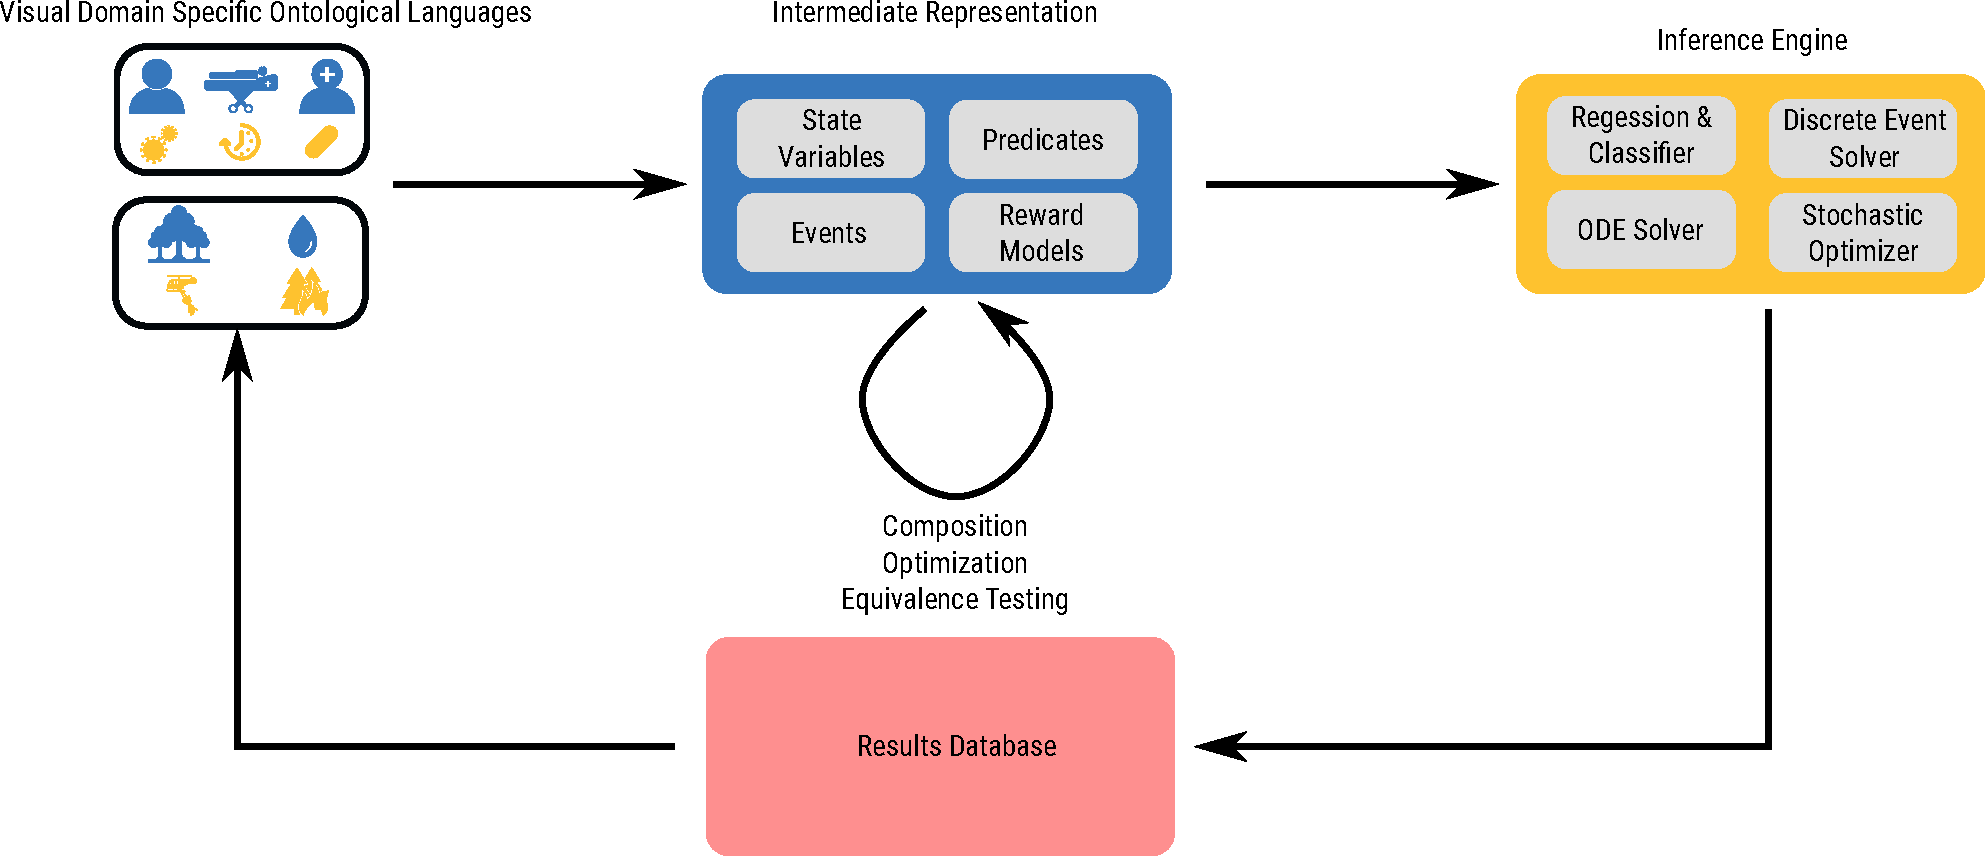
\includegraphics[width=\textwidth]{figs/system-architecture.pdf}
  \caption{\amidol{} architecture.}
  \label{Fig:AMIDOLArch}
\end{figure}

Once a model or models have been defined in a VDSOL, the \amidol{} backend translates the directed graph of nouns and verbs into the \amidol{} intermediate representation, or IR.  The IR is a domain agnostic, universal, modeling formalism.  The \amidol{} backend takes models represented in the IR and can perform model composition to build new models out of two or more existing models, can perform transformations on a model resulting in more performable versions of a model to allow for efficient solution of a model that takes into account structural optimizations, and the necessary requirements to solve a set of reward variables, and can be used to analyze two models to check for the equivalence of two models. The \amidol{} inference engine finally solves a model for a set of defined reward variables, and stores the results obtained in a results database.

The Phase 1 Prototype of \amidol{} implements initial versions of all of these components which are described in the remainder of this report, except the results database and Design of Experiments interface.  During Phase 2 the features of these components will be expanded to full functionality, and the results database and Design of Experiments interface will be implemented.

\section{\amidol{} VDSOL}

\amidol{} is designed to support the definition of ontological languages which describe systems as formal objects.  Objects for a given domain are organized into \emph{palettes} consisting of \textbf{nouns} and \textbf{verbs}.  Nouns define elements which make up the state space of a system, and verbs define transitions in the state space.  VDSOLs enable domain experts to build models of complex systems which are easier to maintain, validate, and verify, and avoid common pitfalls of monolithic and hand-coded implementations.  To provide visual context for modelers, \amidol{} supports the use of arbitrary scalable vector graphics (SVGs) to represent nouns and verbs, and features a canvas to draw nouns and verbs with labeled arcs connecting them to provide context.  Each palette is defined using JavaScript Object Notation (JSON) using a schema which specifies the relevant properties of each known or verb, such as in the following palette for the SIR model:

\begin{lstlisting}[language=json, caption=JSON Definition of SIR VDSOL Palette]
         {"sir" : {
            "population": {
                "className": "population",
                "type": "noun",
                "classDef": "population.air",
                "icon": "images/person.svg",
                "inputVariables": ["P"],
                "outputVariables": ["P"],
                "parameters": [{"name": "P", "value": "0"}]
            }, 
            "patient" : {
                "className": "patient",
                "type": "noun",
                "classDef": "patient.air",
                "icon": "images/patient.svg",
                "inputVariables": ["P"],
                "outputVariables": ["P"],
                "parameters": [{"name": "P", "value": "0"}]
            }, 
            "infect": {
                "className": "infect",
                "type": "verb",
                "classDef": "infect.air",
                "icon": "images/virus.svg",
                "inputVariables": ["S"],
                "outputVariables": ["I"],
                "parameters": [
                    {"name": "beta", "value": "0"},
                    {"name": "total_pop", "value": "0"}
                ]
            },
            "cure": {
                "className": "cure",
                "type": "verb",
                "classDef": "cure.air",
                "icon": "images/cure.svg",
                "inputVariables": ["I"],
                "outputVariables": ["R"],
                "parameters": [{"name": "gamma", "value": "0"}]
            }
        }
\end{lstlisting}

Each noun or verb is given a \texttt{class name}, a \texttt{type} (either noun or verb), a \texttt{class definition} as a pointer to a model in the \amidol{} intermediate representation, an \texttt{icon} to represent the element visually in the editor, and a set of \texttt{input variables}, \texttt{output variables}, and user specifiable \texttt{parameters}.

These definitions create VDSOL elements in an object oriented fashion, declaring nouns and verbs as abstract data types with public, private, and protected methods.  The class as defined in the \amidol{} intermediate representation cannot by default be accessed elements outside of the noun or verb itself, and the \texttt{input variables}, \texttt{output variables}, and \texttt{parameters} are used to expose state variables or events as public or protected members for certain well defined interactions.  The declared set of input variables expose state variables as protected members which can only be accessed by a VDSOL object of the opposite type, and with the same arity, i.e. nouns may only be accessed by verbs and vice versa and then only when cardinality of the input variables of the accessed object exactly match the cardinality of the output variables of the other object.  In Phase 2 these conditions will be relaxed to allow multigraph compositions to provider richer modeling choices and capabilities.  The set of parameters provide public interfaces which the user can specify as constants or expressions to further define interdependencies in a complex system.

The goal of \amidol{}'s VDSOLs is to enable domain experts to define their models using an interface and visual language similar to the semi-formal diagrams they use today, but with the advantage that \amidol{}s VDSOLs have formal, executable, meaning.  VDSOLs provide a performable, reusable, system for scientists to use when attempting to derive insights relating to the complex systems they represent.  Figure \ref{Fig:Palettes} shows example palettes in \amidol{} which are implemented for the Phase 1 prototype.

\begin{figure}
  \begin{subfigure}[b]{\textwidth}
    
\includegraphics[width=\textwidth]{figs/SIR-palette.png}
    \caption{Basic SIR Palette}
    \label{Fig:SIRPalette}
  \end{subfigure}
  \begin{subfigure}[b]{\textwidth}
    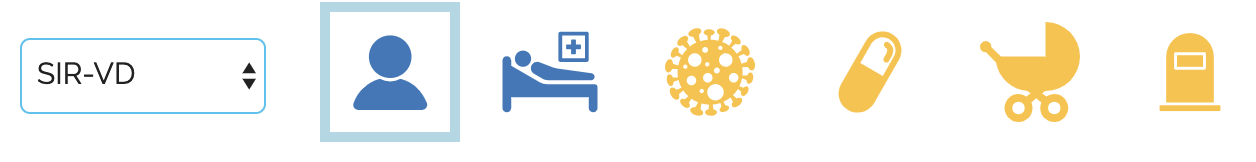
\includegraphics[width=\textwidth]{figs/SIR-VD-palette.png}
    \caption{SIR Palette with Vital Dynamics}
    \label{Fig:SIRVDPalette}
  \end{subfigure}
  \begin{subfigure}[b]{\textwidth}
    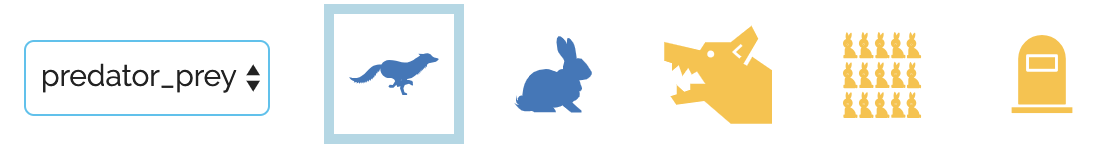
\includegraphics[width=\textwidth]{figs/PREDPREY-palette.png}
    \caption{Lotka–Volterra Predator-Prey Palette}
    \label{Fig:PREDPREYPalette}    
  \end{subfigure}
  \caption{Example \amidol{} Palettes}
  \label{Fig:Palettes}
\end{figure}

\amidol{} is designed to be extended to support any domain through the use of palettes, and to allow researchers to draw diagrams using a visual language that they can modify, extend, and adapt to their needs.  Because these palettes are backed by a universal intermediate representation, they are compatible and comparable even across palettes allowing models developed in differing VDSOLs to be contrasted, analyzed, and even composed.

In Phase 2 these capabilities will be explored with compartmental models for infectious diseases, composing models of populations with limited contact.

\subsection{Structure of \amidol{} VDSOLs}

Formally a VDSOL in \amidol{} is a directed bipartite graph consisting of nodes and edges, with nodes drawn from two classes, nouns and verbs.

\paragraph{Nouns}: Nouns in \amidol{} represent portions of the model associated with its state space, though they may also contain events.  Nouns are represented by custom SVGs, and can be connected to verbs which act upon them.  Users can set the label associated with a noun, which impacts the naming of state variables and events associated with the noun, and set the value of any parameters exposed through the VDSOL parameter property allowing the nouns to be specialized with initial conditions, constants, or expressions.

\paragraph{Verbs}: Verbs in \amidol{} represent changes in the state of the model, and which conceptually act upon nouns.  Like nouns they contain state variables, unlike nouns they must also contain events.  The state variables in a verb may be used to track state dependent rates, or internal properties, but also to define the side effects of the verb.  A verb's input variables and output variables are used to connect verbs to nouns through composition.

\subsection{Composability of Atomic Models}

\amidol{} is being designed to support the composition of individual models in Phase 2 to enable model reuse, compositional methods for solution, to enhance backend support for performance optimizations that require symmetry detection, and to allow domain scientists to experiment by swapping out components of a model which may represent complex hypotheses about individual elements.  Model composition in \amidol{} is being designed to support two primary mechanisms: \emph{state-sharing} \cite{sanders1992dependability,sanders1988construction} and \emph{event-synchronization} \cite{lampka2002symbolic}.

Composition is currently partially implemented in the Phase 1 prototype, as it is employed as the method for building the IR model from the underlying definitions of nouns and verbs connected in the UI.  In Phase 2 a model composition editor will be added to the UI to allow composing via state-sharing. State-sharing allows model composition by defining an interface for a model in the form of a set of state variables, which are then "shared" with another model.  Shared state-variables in two composed models have the same marking, or value, and are effected by events in both models.  Event-synchronization functions in an analogous way, allowing two events to be paired, such that the input predicate and output predicate of the new shared event is the union of the predicates of the events being shared.

\amidol{} will support replicate and join operations previously defined over Petri-nets and stochastic activity networks, but extended to the \amidol{} IR. \cite{sanders1995ultrasan}  In addition to replicate and join operations, \amidol{} will support a novel model composition relation allowing users to specify sub-models as nouns and verbs which can be connected to existing components using Abstract Base Models, based on class inheritance patterns \cite{bruce2002foundations}, which allows users to specify abstract models with undefined states and events.

\section{\amidol{} Intermediate Representation}

The Abstract Intermediate Representation (IR) for \amidol{} is meant to be a universal way to specify models, regardless of their domain, and provides a Turing-complete way to specify models performably, while avoiding domain specific considerations.  Models are defined in the IR for \amidol{} using JSON for serialized representations using the following schema:

\begin{lstlisting}[language=json, caption=JSON Schema for the AMIDOL Intermediate Representation]
{ "irModel": {
  "irModelName": "string",
  "stateVariables": [{
    "name": "string",
    "label": "string",
    "type": "sv_type",
    "initial_value": "expression"
  }],
  "events": [{
    "name": "string",
    "label": "string",
    "rate": "expression",
    "input_predicate": {
      "enabling_condition": "expression"
    },
    "output_predicate": {
      "transition_function": ["lvalue = expression", "lvalue = expression", ...]
    }
  }],
  "constants": [{
    "name": "string",
    "value": "extern"|"expression"
  }],
  "expressions": [{
    "name": "string",
    "value": "extern"|"expression"
  }],
  "rateRewards": [{
    "name": "string",
    "variable": "string",
    "temporaltype": "instantoftime"|"intervaloftime"|"timeaveragedintervaloftime"|"steadystate",
    "samplingpoints": [{
      "time": "float"
      }]    
  }],
  "impulseRewards": [{
    "name": "string",
    "event": "string",
    "temporaltype": "instantoftime"|"intervaloftime"|"timeaveragedintervaloftime"|"steadystate",
    "samplingpoints": [{
      "time": "float"
      }]    
  }],
  "composedrewards": [{
    "name": "string",
    "expression": "expression"
  }]
}}
\end{lstlisting}

The \amidol{} backend performs transformations on models defined in this IR allowing it to act on models via well structured transformations as shown in Figure \ref{Fig:AMIDOLBackend}.  Even though we have not implemented the Model Composition editor for Phase 1, the backend composition operators have been implemented in our prototype as they form the basic operation needed to combine nouns, verbs, and reward variables into an executable model.  The design principles used for the backend focus on this concept of reusable operations which enable complex interactions and features.

\begin{figure}
  \begin{eqnarray}
    \mathrm{translate}(\mathrm{VDSOL}_A) & \rightarrow & \mathrm{IR}_A\\
    \mathrm{compose}(\mathrm{IR}_A, \mathrm{IR}_B) & \rightarrow & \mathrm{IR}_C\\
    \mathrm{translate}(\mathrm{IR}_A) & \rightarrow & \mathrm{target}_A\\
    \mathrm{optimize}(\mathrm{IR}_A)) & \rightarrow & \mathrm{IR}_B\\
    \mathrm{equivalence}(\mathrm{IR}_A, \mathrm{IR}_B) & \rightarrow & \mathrm{True} \vee \mathrm{False}
  \end{eqnarray}
  \caption{}
  \label{Fig:AMIDOLBackend}
\end{figure}

Currently the Phase 1 prototype implements only the \texttt{translate} and \texttt{compose} functionality shown in Figure \ref{Fig:AMIDOLBackend}, but in Phase 2 we will extend \amidol{} to account for all of this proposed functionality.  A core goal of \amidol{} is to use the intermediate representation to abstract away a lot of the details of target translations for solution, including necessary performance optimizations, conditions for solutions, and requirements of solution targets.

The intermediate representation employed by \amidol{} has its roots in Markov models \cite{howard2012dynamic}, Generalized Stochastic Petri-nets with inhibitor arcs \cite{chiola1993generalized} (which have been shown to be Turing complete), and stochastic activity networks \cite{movaghar1985performability,sanders2000stochastic} (an extension of Petri-nets that allow more compact model specification).  \amidol{} currently extends these concepts primarily by creating ways to link to the original ontology of nouns and verbs, and by allowing embedded reward structures to be linked to a graph-based results database which stores the outcomes of experiments and can be used for the construction of arbitrary measures on the underlying model to support inference needs.


\subsection{Language Properties}

Formally, the IR is a 5-tuple, $(S, E, L, \Phi, \Lambda, \Delta)$ where:
\begin{itemize}
\item $S$ is a finite set of state variables $\{s_0, s_1, \ldots, s_{n-1}\}$ that take on values in $\mathbb{N}$.
\item $E$ is a finite set of events $\{e_0, e_1, \ldots, e_{m-1}\}$ that may occur in the model.
\item $L: S|E \rightarrow \mathbb{N}$ is the event and state variable labeling function that maps elements of $S$ and $E$ into the original ontology.
\item $\Phi: E \times N_0 \times N_1 \times \ldots \times N_{n-1} \rightarrow \{0, 1\}$ is the event enabling predicate.
\item $\Lambda: E \times N_0 \times N_1 \times \ldots \times N_{n-1} \rightarrow (0, \infty)$ is the transition rate specification.
\item $\Delta: E \times N_0 \times N_1 \times \ldots \times N_{n-1} \rightarrow N_0 \times N_1 \times \ldots \times N_{n-1}$ is the state variable transition function specification.
\end{itemize}

Informally the IR represents models defined in a given VDSOL using an formalism based on Generalized Stochastic Petri-nets with inhibitor arcs (which have the result of making Petri-nets Turing complete).  Instead of inhibitor arcs, we utilize the more intuitive and performable method of allowing events to have input predicates ($Phi$) which can be evaluated to determine if an event is enabled, and output predicates which define the side effects of event firing.

\paragraph{State variables}: intuitively, state-variables make up the current state of the model, and measure the configuration and capabilities of all modeled components.  While state variables are defined as taking on values in $\mathbb{N}$, this does not restrict them from representing real numbers to arbitrary precision in modern computer hardware.  In practice, they are implemented as integers, and floating point numbers by the \amidol{} source code.

\paragraph{Events}: events, when fired, change the state of a model by altering the value of state variables.  Events in \amidol{} are associated with input predicates, output predicates, and a rate function which returns the next firing time of a given event.  The rate function is an expression over random variable distributions.

\paragraph{Input predicates}: an input predicate is associated with an event, and a potentially empty set of state variables.  Input predicates are functions of the marking of their set of variables which map the markings of those variables onto the set $\{1, 0\}$.  For those markings in which the input predicate evaluates to $1$, the event is considered enabled and will fire as normal.  For those markings in which the input predicate evaluates to $0$, the event is considered disabled and cannot fire until subsequently enabled.

\paragraph{Output predicates}: an output predicate is associated with an event, and a potentially empty set of state variables.  Output predicates map a set of state variables, and their marking, to a new marking for the same state variables and define the side effects of event firing on the state of the model.

\section{\amidol{} Reward Variables}

The \amidol{} intermediate representation allows for the specification of reward variables or structures over a given model, and the composition of these structures with a model to produce composed models which can then be solved by the inference engine.  Given a model $M = (S, E, L, \Phi, \Lambda, \Delta)$ we define two basic types of rewards structures, rewards over state variable values (rate rewards), and rewards over events (impulse rewards). \cite{qureshi1996algorithms,deavours1999efficient,ciardo1996well,sanders1991reduced}

In Phase 1 we have only implemented reward variables, as a performable discrete event solver is required to fully validate an implementation of impulse reward variables (whose solution is otherwise trivial for numerical methods).  During Phase 2 we will rapidly identify a discrete event solver as a backend target, and include impulse rewards as an early stage Phase 2 goal and deliverable.

\subsection{Rate Reward Variables}

A rate reward is formally defined as a function $\mathcal{R}: P(S, \mathbb{N}) \rightarrow \mathbb{R}$ where $q \in P(S, \mathbb{N})$ is the reward accumulated when for each $(s,n) \in q$ the marking of the state variable $s$ is $n$.  Informally a rate reward variable $x$ accumulates a defined reward whenever a subset of the state variables take on prescribed values.

\subsection{Impulse Reward Variables}

An impulse reward is formally defined as a function $\mathcal{I}: E \rightarrow \mathbb{R}$ where $e \in E, \mathcal(I)_e$ is the reward for the completion of $e$.  Informally an impulse reward variable $x$ accumulates a defined reward whenever the event $e$ fires. Impulse rewards will be implemented in Phase 2, when the backend targets currently offered are expanded to include a performable discrete event simulator.

\subsection{Temporal Characteristics of Reward Variables}

Both rate and impulse reward variables measure the behavior of a model $M$ with respect to time.  As such, a reward variable $\theta$ is declared as either an instant-of-time variable, an interval-of-time variable, a time-averaged interval-of-time variable, or a steady state variable.  An instant of time variable $\Theta_t$ is defined as:

\[ \theta_t = \sum_{\nu \in P(S, \mathbb{N})} \mathcal{R}(\nu) \cdot \mathcal{I}^{\nu}_t + \sum_{e \in E} \mathcal{I}(e) \cdot I_t^e\]

Intuitively a rate reward declared as an instant-of-time variable \cite{freire1990technique} can be used to measure the value of a state variable precisely at time $t$, and an impulse reward declared as an instant-of-time variable can be used to measure whether a given event fired at precisely time $t$.  While the latter is not a particularly useful measure (as the probability of an event with a firing time drawn from a continuous distribution at time $t$ is $0$) it is defined for closure reasons, and for cases with discrete distributions and discrete time steps.

An interval-of-time variable intuitively accumulates reward over some fixed interval of time $[t, t+1]$.  Given such a variable $\theta_{[t, t+1]}$ we formally define interval-of-time variables as:

\[\theta_{[t,t+1]} = \sum_{\nu \in P(S, \mathbb{N})} \mathcal{R}(\nu) \cdot \mathcal{J}^{\nu}_{[t, t+1]} + \sum_{e \in E} \mathcal{I}(e)N^e_{[t,t+1]}\]

where

\begin{itemize}
\item $J^{\nu}_{[t,t+1]}$ is a random variable which represents the total time the model spent in a marking such that for each $(s, n) \in \nu$, the state variable $s$ has a value of $n$ during the period $[t, t+1]$.
\item $I^e_{t\rightarrow\infty}$ is a random variable which represents the number of times an event $e$ has fired during the period $[t, t+1]$.
\end{itemize}

Time-averaged interval of time variables quantify accumulated reward over some interval of time.  Such a variable $\theta'_{[t,t+1]}$ is defined formally as:

\[\theta'_{[t,t+1]} = \frac{\theta_{[t,t+1]}}{l}\]

Steady state reward variables are realized by testing for initial transients, and calculating an instant of time variable after a model has reached a stable steady state with high confidence.

For Phase 1 we have focused on instant of time variables.  During Phase 2 we will implement interval of time and steady state reward variables.  Steady state reward variables will make heavy use of our ability to perform transformations on the IR, as they represent an often wholly different solution target.

\subsection{Composed Reward Variables}

A key target of Phase 2 for \amidol{} will be extension of reward variables to allow composed rewards, which are expressions defined over other reward variables allowing us to construct a set of arbitrary measures on the set of atomic, and universal, measures of rate and impulse rewards. While individual reward variables form the basis for model evaluation, \amidol{} will support expressions defined over reward variables using basic arithmetic operations allowing reward variables to be composed via normal mathematical expressions.

\section{Design of Experiments and Results Database}

\begin{figure}
  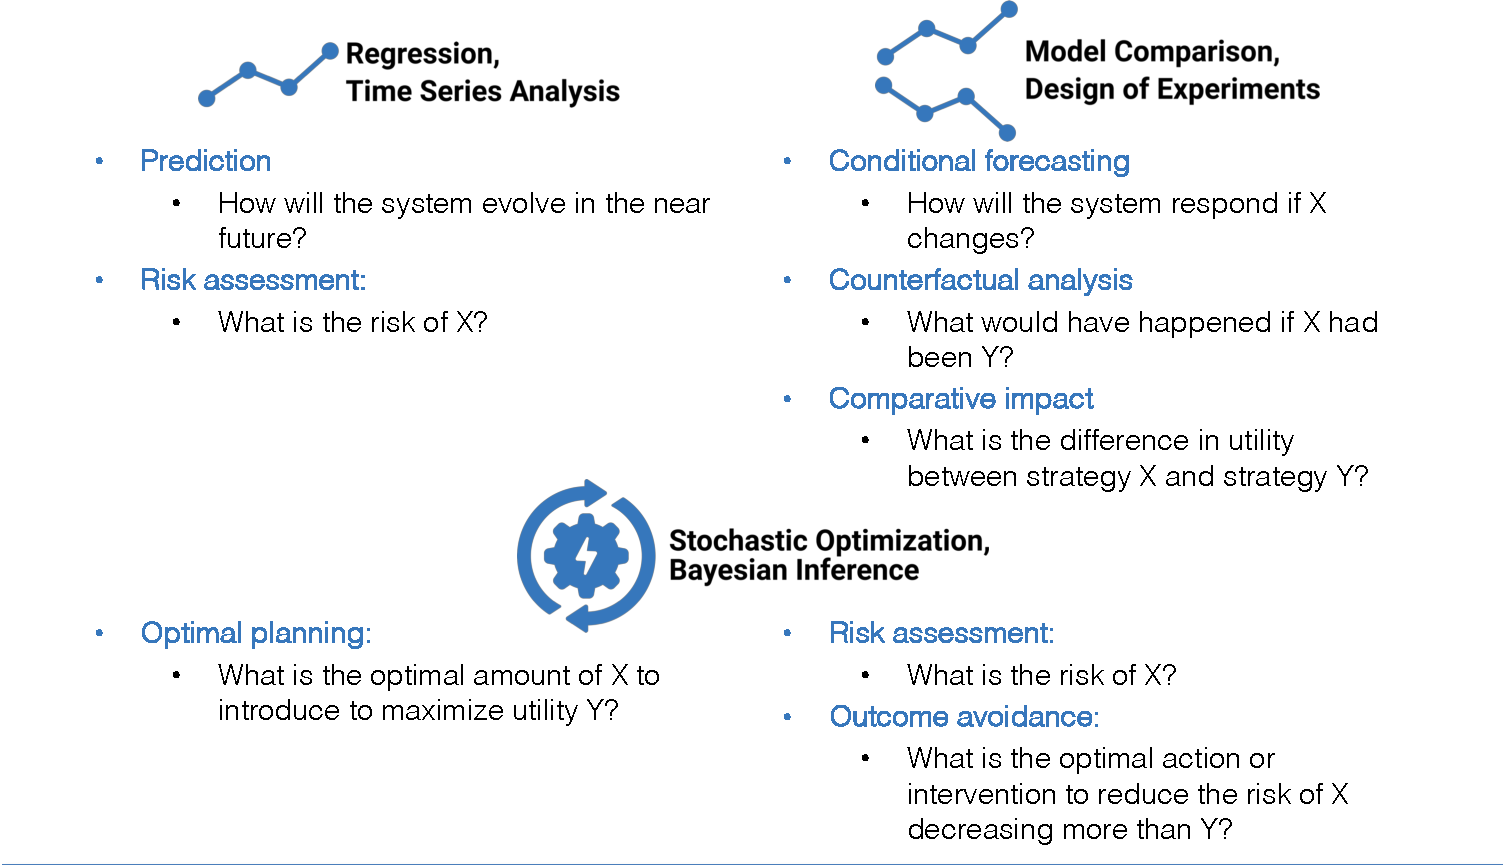
\includegraphics[width=\textwidth]{figs/table.pdf}
  \caption{}
  \label{Fig:InferenceClasses}
\end{figure}

During Phase 2, a key extension of \amidol{} will be the implementation of a Design of Experiments interface \cite{montgomery2017design}, coupled with a results database in order to support the complex queries and prognostics, as shown in Figure \ref{Fig:InferenceClasses}, required of the program.  Design of Experiments in \amidol{} will borrow from concepts of Plackett-Burman designs, and factorial designs using individual reward variables and parameterizations defined over a given model as atomic components of expressions.  Computations for given atomic components will be stored in the results database to avoid unneeded reevaluation, and to allow future experiments to build on past results, and be directly compared and contrasted.

The Design of Experiments interface will also allow users to load data from external sources, and associate this data with expectations for state variables in the model.  In our early tests we have achieved this by using data from the CDC's Fluview \cite{cdc2019fluview} data sets as series of instant-of-time observations.  \amidol{}'s interface will allow users to use regression to estimate the conditional expectation of dependent variables, given independent variables with fixed values from the data, allowing prediction, parameter estimation, and later risk assessment for a given regression through analysis of the distribution of possible realizations for state variables in a given model.

The planned Design of Experiments interface will allow direct comparison through user identification of reward variables, or expressions on reward variables, in two models which represent comparable properties or processes allowing the exploration of alternatives, conditional forecasting, counterfactual analysis, and comparative impact.  Different strategies, configurations, or possible outcomes can be explored through examining different ways to parameterize a given model, or even differences in models with structural changes.  Debugging experiments will be enabled through the connections to the VDSOL ontology.  For instance, the interface will allow users to see the direct dependence of reward variables to noun's and verbs in the original ontology, better enabling researchers to understand the knowledge-based semantic dependencies normally hidden by traditional modeling techniques.

Sensitivity, uncertainty, and correctness measures can easily be constructed in the planned Design of Experiments interface.  Because we allow for factorial and Plackett-Burman experiment design users can automatically perform one-factor-at-a-time \cite{bailis2005mortality,murphy2004quantification} sensitivity and uncertainty estimates.  The initial prototype will also feature screening sampling-based methods \cite{morris1991factorial} which have been shown to be computationally efficient and are further enabled by our VDSOL ontologies, as they help identify sources of uncertainty and error in the structure of the model.  Correctness is enabled by loading external data from multiple time series or sources, and asking the interface to perform cross validation on the input.  \amidol{} will automatically support k-fold cross validation on time series, allowing automatic partitioning of data sets.

\section{\amidol{} Inference Engine}

The Phase 1 prototype of \amidol{} supports two solver targets for the intermediate representation PySCeS: the Python Simulator for Cellular Systems \cite{olivier2011pysces,olivier2005modelling}, an extendable toolkit for analyzing compartmental systems, and through the use of the SciPy odeint functionality to simulate an ordinary differential equation based representation of a model in the IR \cite{oliphant2004scipy,ahnert2011odeint}.  These targets were chosen both for reasons of validation, since they produce comparable output, but also as a proof of concept given their very different target languages.

The PySCeS solver has its own internal language which is used to specify compartmental models.  \amidol{} supports this backend by providing a translation from the IR into the PySCeS specification language, and then invoking PySCeS on the translation.  We illustrate a translation here by showing the outputs of \amidol{} for the basic SIR model in PySCeS:

\begin{verbatim}
Modelname: tmp_model
Description: Autogenerated tmp_model

Species_In_Conc: False
Output_In_Conc: False

# Reactions
reaction_4:
     Infected > Recovered
     0.333 * Infected

reaction_2:
     Susceptible > Infected
     0.413 * Susceptible * Infected / 
        (Susceptible + Infected + Recovered)


# Parameter values
Recovered = 250.0
Susceptible = 250.0
Infected = 250.0
Example = 0.0
\end{verbatim}

The SciPy odeint solver target is supported through a similar method by \amidol{}.  A translation is provided from the IR into a Python script which includes and invokes SciPy's odeint solver for ordinary differential equations.  The IR model is then represented directly as a system of ordinary differential equations for solution.  We show here the same model previously generated for PySCeS as generated by \amidol{} for SciPy odeint:

\begin{lstlisting}[language=python]
from scipy.integrate import odeint
import json
import numpy as np
import matplotlib.pyplot as plt

class NumpyEncoder(json.JSONEncoder):
    def default(self, obj):
        if isinstance(obj, np.ndarray):
            return obj.tolist()
        return json.JSONEncoder.default(self, obj)

# User defined constants
Example = 0.0

# The ODE system
def deriv_(y_, t_):
    Recovered, Susceptible, Infected = y_
    dInfected_ = 0.0 - 0.333 * Infected + 0.413 * Susceptible * Infected /
       (Susceptible + Infected + Recovered)
    dRecovered_ = 0.0 + 0.333 * Infected
    dSusceptible_ = 0.0 - 0.413 * Susceptible * Infected /
       (Susceptible + Infected + Recovered)
    return dRecovered_, dSusceptible_, dInfected_

# Boundary conditions and setup
timeRange_ = [ 0.0, 5.0, 10.0, 15.0, 20.0, 25.0, 30.0, 35.0, 40.0, 45.0, 50.0,
55.0, 60.0, 65.0, 70.0, 75.0, 80.0, 85.0, 90.0, 95.0 ]
y0_ = 250.0, 250.0, 250.0
output = odeint(deriv_, y0_, timeRange_).T

print(json.dumps(output, cls=NumpyEncoder))
\end{lstlisting}

\amidol{}'s backend inference engine is designed to support a wide range of inference techniques as build targets chosen by the intermediate representation based on the requirements of the reward variables being computed, and the limitations and requirements of the models being solved.  A model, for instance, which has general event distributions, cannot be solved by successive matrix multiplication; the distribution of a reward variable can likewise not be computed by solving the underlying system of differential equations.

The strength of \amidol{} is this decoupling of modeling and representational concerns from the choice of executable implementation. \amidol{} removes these concerns from the domain expert, and automates these translations, allowing arbitrary modifications to be performed on the visual model, and rapid iteration of model structure, and parameters while exploring hypothesis, or comparing a model to actual data.  While \amidol{} doesn't prevent a user from making mistakes while modeling, it reduces the occurance of implementation details, and helps users to more rapidly design and prototype models by removing abstract concerns, and details such as choice of language, or unfamiliar requirements of solution methods.  While some work must be done to adapt \amidol{} to support a new solver target, once accomplished it can be leveraged for any VDSOL, allowing easy collaboration, and an ability to build on the work of others in a generalizable way.

A key feature for Phase 2 of \amidol{} will be the use of multiple solvers and techniques on the same model to compute different reward variables where appropriate, with the results being fed into a results database.  This  backend architecture helps to ensure the performability of models designed in \amidol{}, and flexibility of solution technique helping researchers avoid the pitfall of being bound to a single target using hand coded models, which may or may not be performable.


\section{Domain Models}

We are currently testing \amidol{} using several domain models.  We have selected a range of models to test different scenarios, use cases, and assumptions to aid in the prototype design of \amidol{}.

\subsection{SIS/SIRS}

The SIS/SIRS model is one of the simplest models we have deployed for testing with \amidol{}, with the advantage that the model itself is relatively simple, but utilizes real data, and can be used to answer important epidemiological questions.  The primary objective of the SIS/SIRS model is to identify the \emph{basic reproduction number} associated with an infection, also known as $R_0$, or \emph{r nought}.  $R_0$ was first used in 1952 when studying malaria and is a measure of the potential for an infection to spread through a population.  If $R_0 < 1$, then the infection will die out in the long run.  If $R_0 > 1$, then the infection will spread.  The higher the value of $R_0$, the more difficult it is to control an epidemic.

The importance of estimating $R_0$ has been well established for many historical epidemics, including H1N1 \cite{fraser2009pandemic} and Ebola \cite{fisman2014early}.  This model also lends itself to testing \amidol{}'s Design of Experiments module via the plentiful CDC Data \cite{cdc2019fluview} which is well modeled by SIRS.

Given a 100\% effective vaccine, the proportion of the population that needs to be vaccinated is $1 - 1/R_0$, meaning that $R_0$ can be used to plan disease response.  This assumes a homogenous population, and contains many other simplifying assumptions and does not generalize to more complex numbers.  We have several main goals for SIS/SIRS models:

\begin{enumerate}
\item Fitting the models for the data in hindsight to perform goodness of fit estimates.
\item Finding the \emph{retrospective} $R_0$ estimate over the entire epidemic curve.
\item Finding the \emph{real-time} $R_0$ estimate while the epidemic is ongoing.
\end{enumerate}

\paragraph{Data}: For these models we have worked with the WHO/NREVSS (World Health Organization/National Respiratory and Enteric Virus Surveillance System) data sets at the resolution of Department of Human and Health Services designated regions.

\begin{figure}

\includegraphics[width=\textwidth]{figs/regionsmap.pdf}
\caption{Department of Human and Health Services designated regions.}
\label{Fig:Regions}
\end{figure}

Using data from a given region, and a given strain, we estimate R0 for the epidemic curve as shown in Figure \ref{Fig:R0}

\begin{figure}
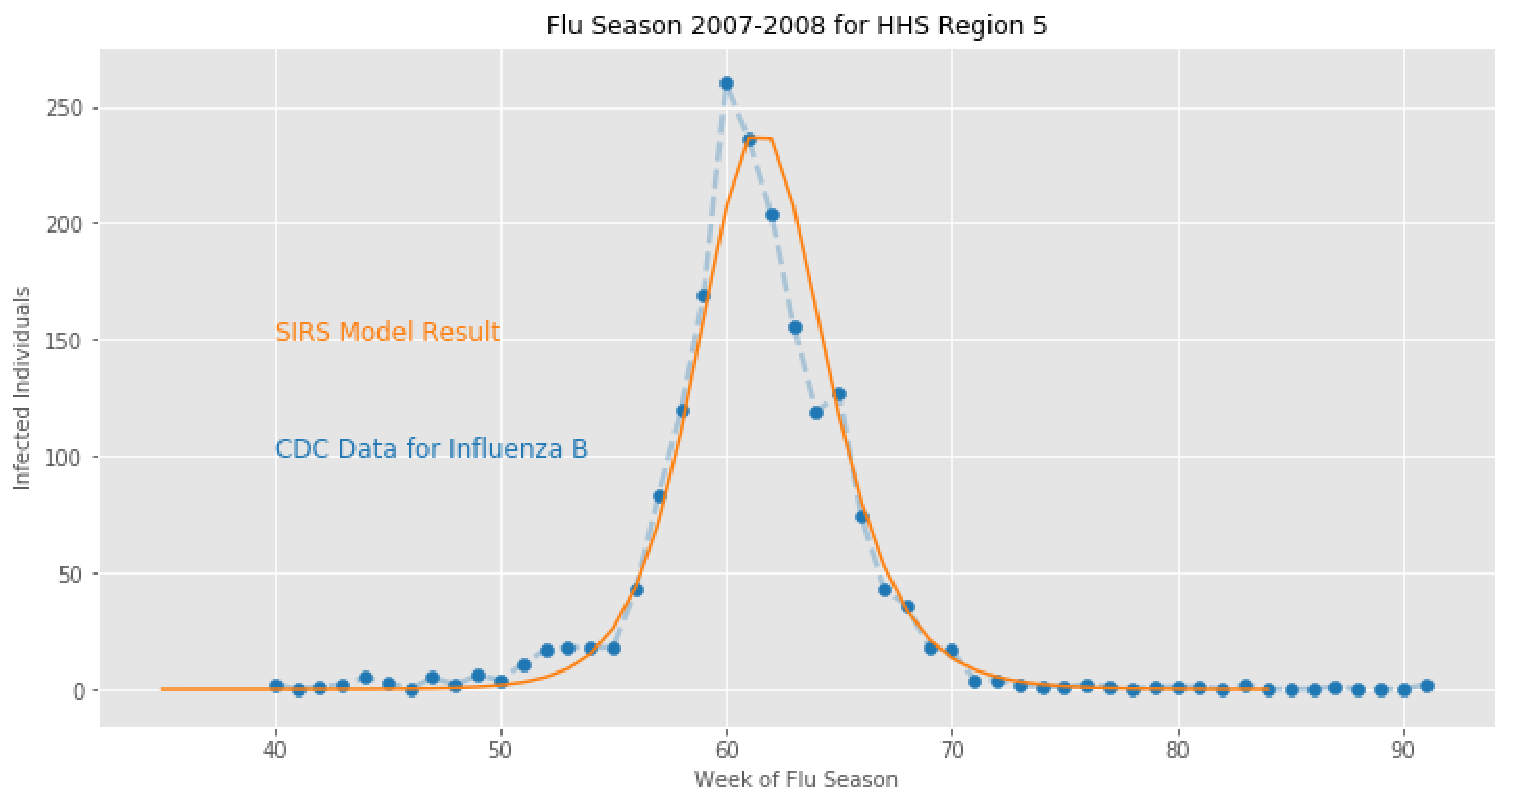
\includegraphics[width=\textwidth]{figs/2007-2008-SIRS.pdf}
\caption{2007 - 2008 Flu Season}
\label{Fig:R0}
\end{figure}

\subsection{SIS/SIRS with Vital Dynamics}

Extending the SIRS model, we also include an example of palette extension.  The palettes defined for \amidol{} can be modified, and even extended, easily by adding new nouns and verbs.  This allows for the long term curation of models by domain experts, who can easily extend their earlier work as new processes and interactions are discovered.  The Vital Dynamics modification of SIRS allows the definition of models in which new individuals are born into populations, and for individuals to be removed from populations due to death from various causes.  Increasesing the rate of infected populations dying, when compared to susceptible and recovered populations, also allows modeling a potentially lethal disease.

\begin{figure}
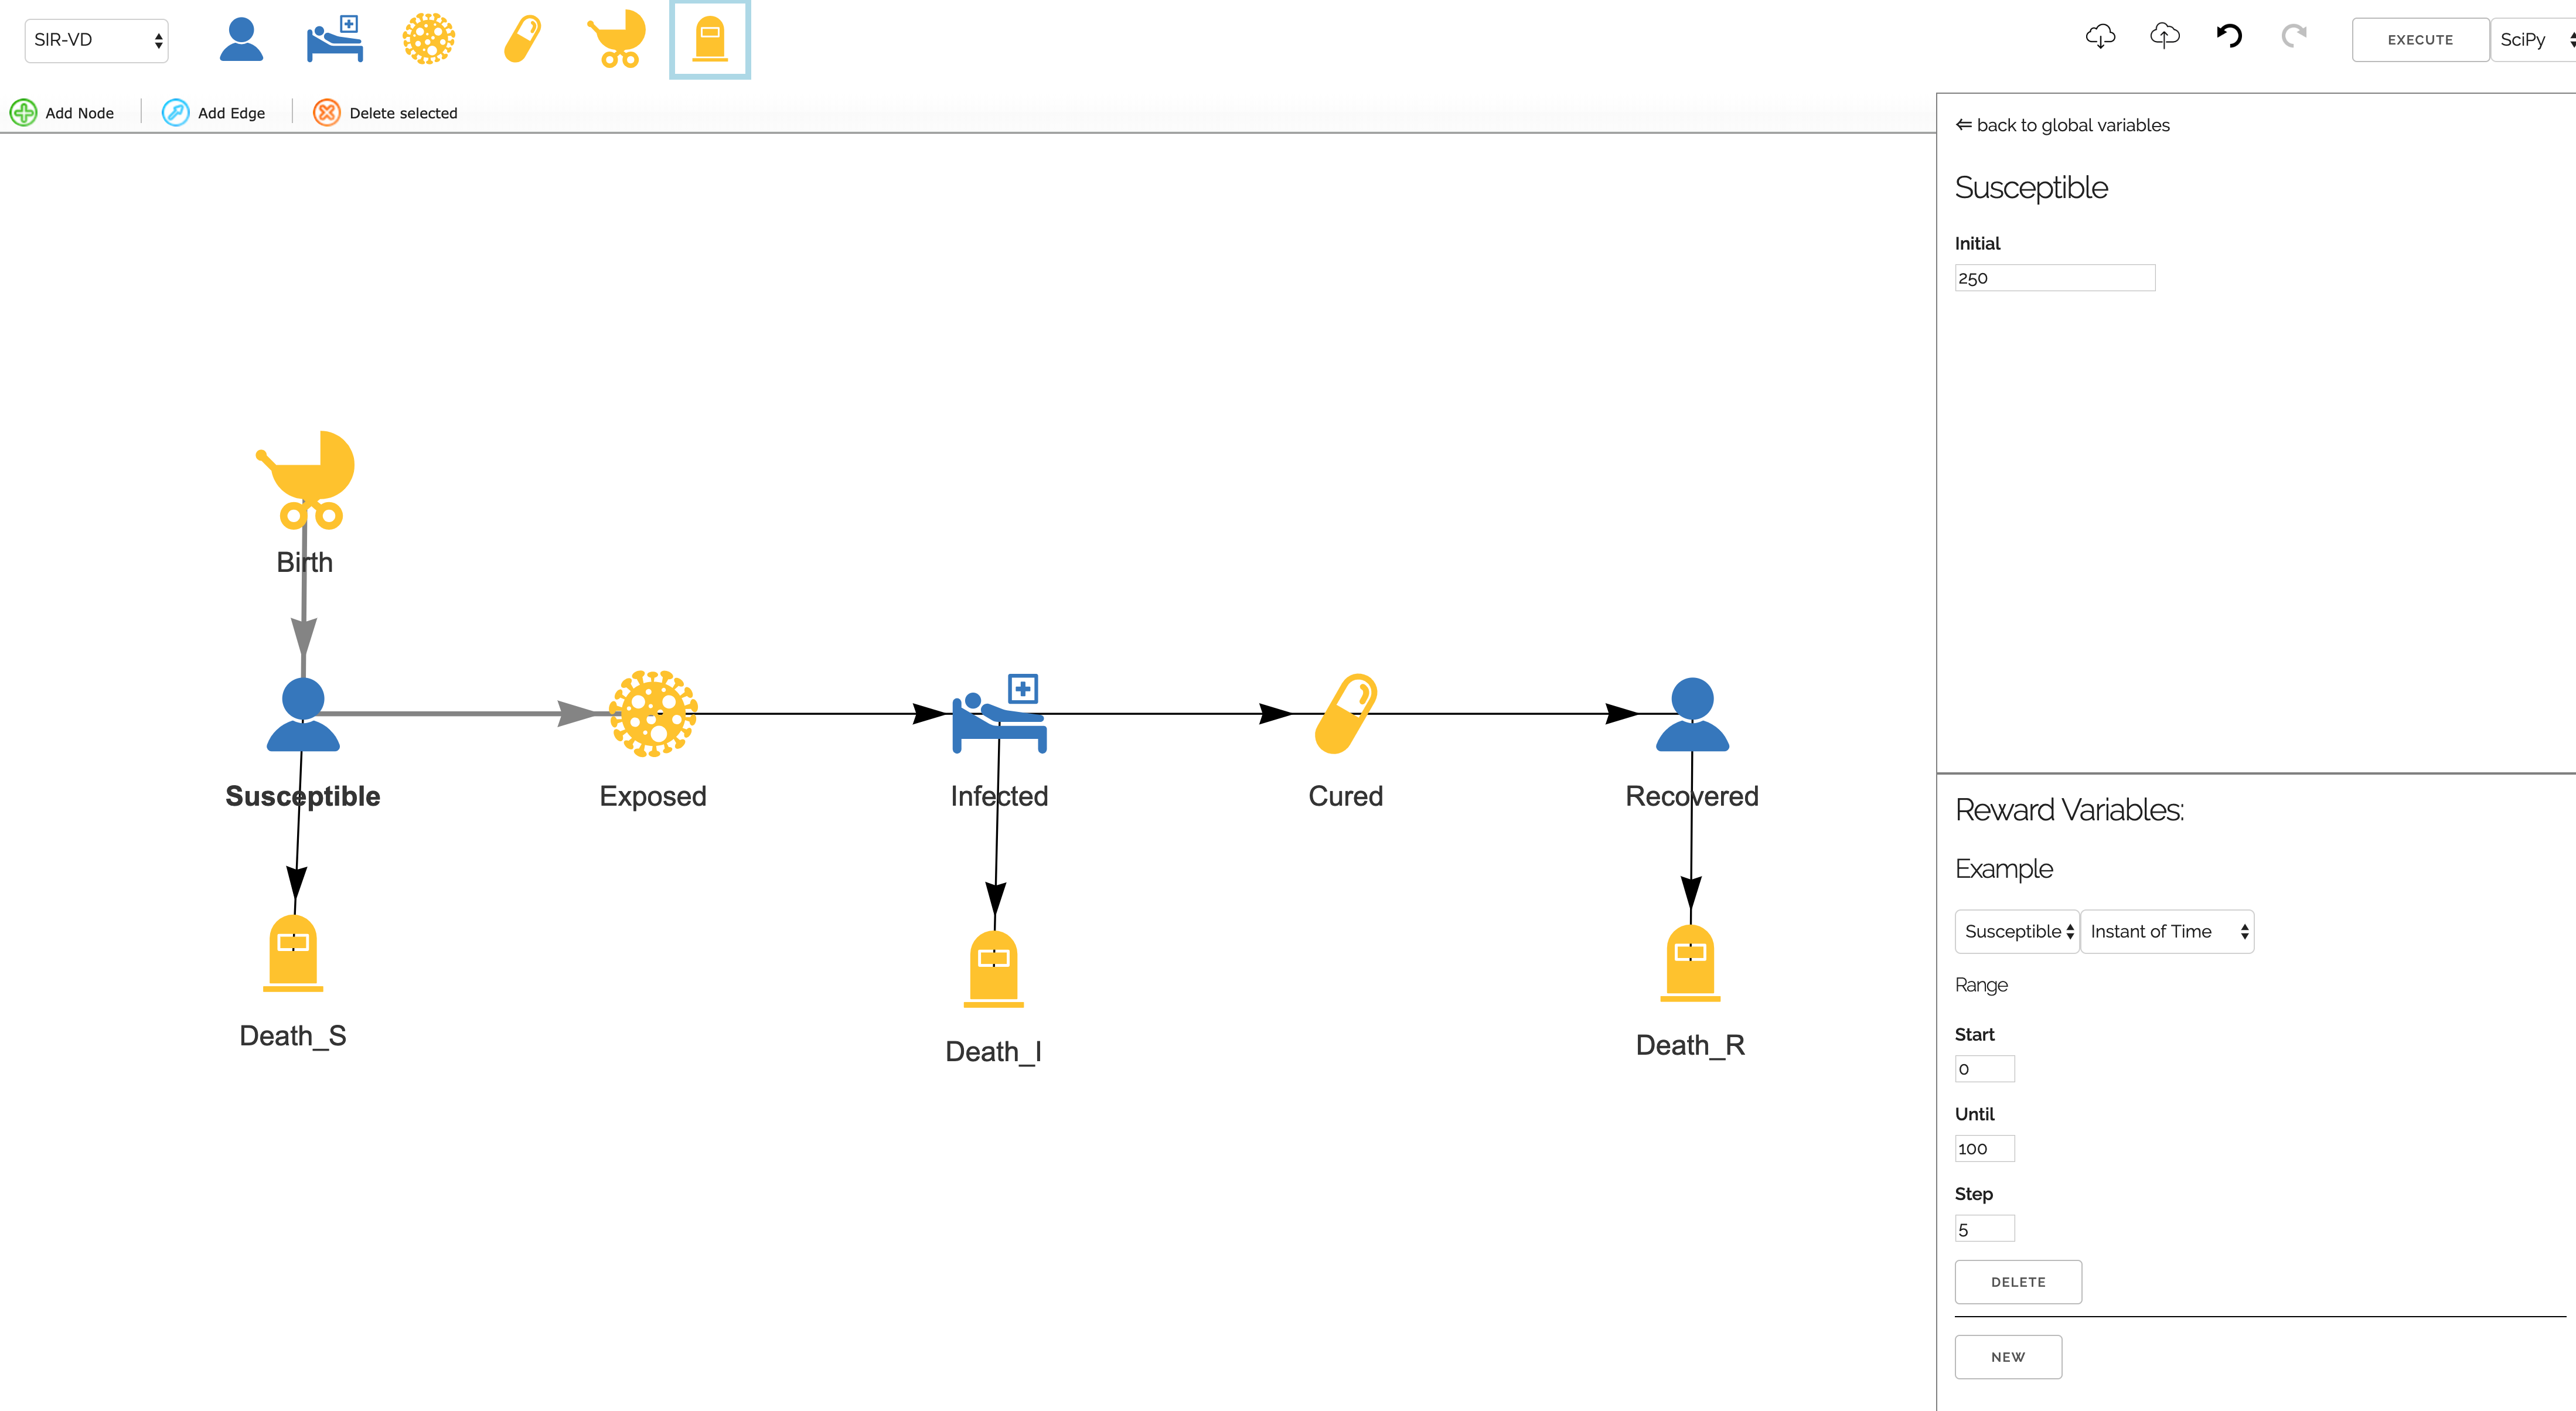
\includegraphics[width=\textwidth]{figs/SIR-VD.png}
\caption{SIR Model with Vital Dynamics}
\label{Fig:SIR-VD-Draw}
\end{figure}

The following equations show the typical modification of the ordinary differential equations used to represent a SIR model with vital dynamics:

\begin{eqnarray}
  \frac{dS}{dt} &=& \mu N - \frac{\beta S I }{N} - \nu S\\
  \frac{dI}{dt} &=& \frac{\beta S I}{N} - \gamma I - \nu I\\
  \frac{dR}{dt} &=& \gamma I - \nu R
\end{eqnarray}

While these equations convey the underlying mathematical meaning of the model, their intuitive and semantic meaning is somewhat opaque.  Figure \ref{Fig:SIR-VD-Draw} shows the implementation of this model in \amidol{}'s SIR-VD palette.  The result is a diagram that mirrors the sort of semi-formal diagram which has intuitive meaning to a domain expert and also has the same mathematical meaning as the system of equations due to \amidol{}'s ability to perform a direct translation to the same underlying model.

\subsection{Lotka-Volterra Model}

As an example of a wholly different palette for a VDSOL, and to demonstrate the capability of our Phase 1 prototype to handle models in different domains, we have also implemented a domain model for the Lotka-Volterra model of predator-prey relationships \cite{freedman1980deterministic,brauer2012mathematical,hoppensteadt2006predator}.  Frequently used to describe the basic dynamics of biological systems with two species interactions, the Lotka-Volterra model assumes a single predator, and single prey species.  While a simple model, this system is an example of a Kolmogorov model which is used as the underlying framework for modeling other dynamic systems, such as competing species in a niche, the impact of disease on a species, and mutalistic relationships.  It is provided in our initial prototype primarily as another model for which it is easy to validate and generate expectations, and to demonstrate the capacity of our prototype to work in multiple domains.

\section{Code Repositories and Current Builds}

The Phase 1 \amidol{} prototype is available, along with all source code in our repository with instructions on building and executing the current system.  Models can be designed in the current VDSOL editor, a javascript front-end.  The intermediate representation is implemented as a Scala project which compiles queries issued by users for a particular model they've created into code artifacts targeting different solver backends. Over time, we expect this system to also manipulate and compose datasets (from real-world observations as well as from the output of other simulations), and utilize the results database to save intermediate results and compare evaluations and models.

\subsection{Front-End Architecture}

\amidol{}'s user interface is currently implemented using HTML, CSS, and Javascript, communicating with the Scala back-end using JSON over HTTP.  This client/server approach leverages standard browser technologies for rapid development of rich interactions tailored for the specific needs of scientific modeling. It also decouples the concerns of visual presentation and manipulation from the underlying representations of model semantics and helps to hide the details from domain experts reducing their cognitive load when designing models.

The current user interface implements a rich visual editor allowing users to select a palette to work in, to save and load VDSOL diagrams, undo and redo operations, to customize parameters exposed by nouns and verbs, to define reward variables on a diagram, and to call multiple backend solver targets to solve those reward variables.
Currently, the user interface implements a visual editor for directed graphs having labeled vertices and edges, which represent the nouns and verbs of a VDSOL.

\begin{figure}
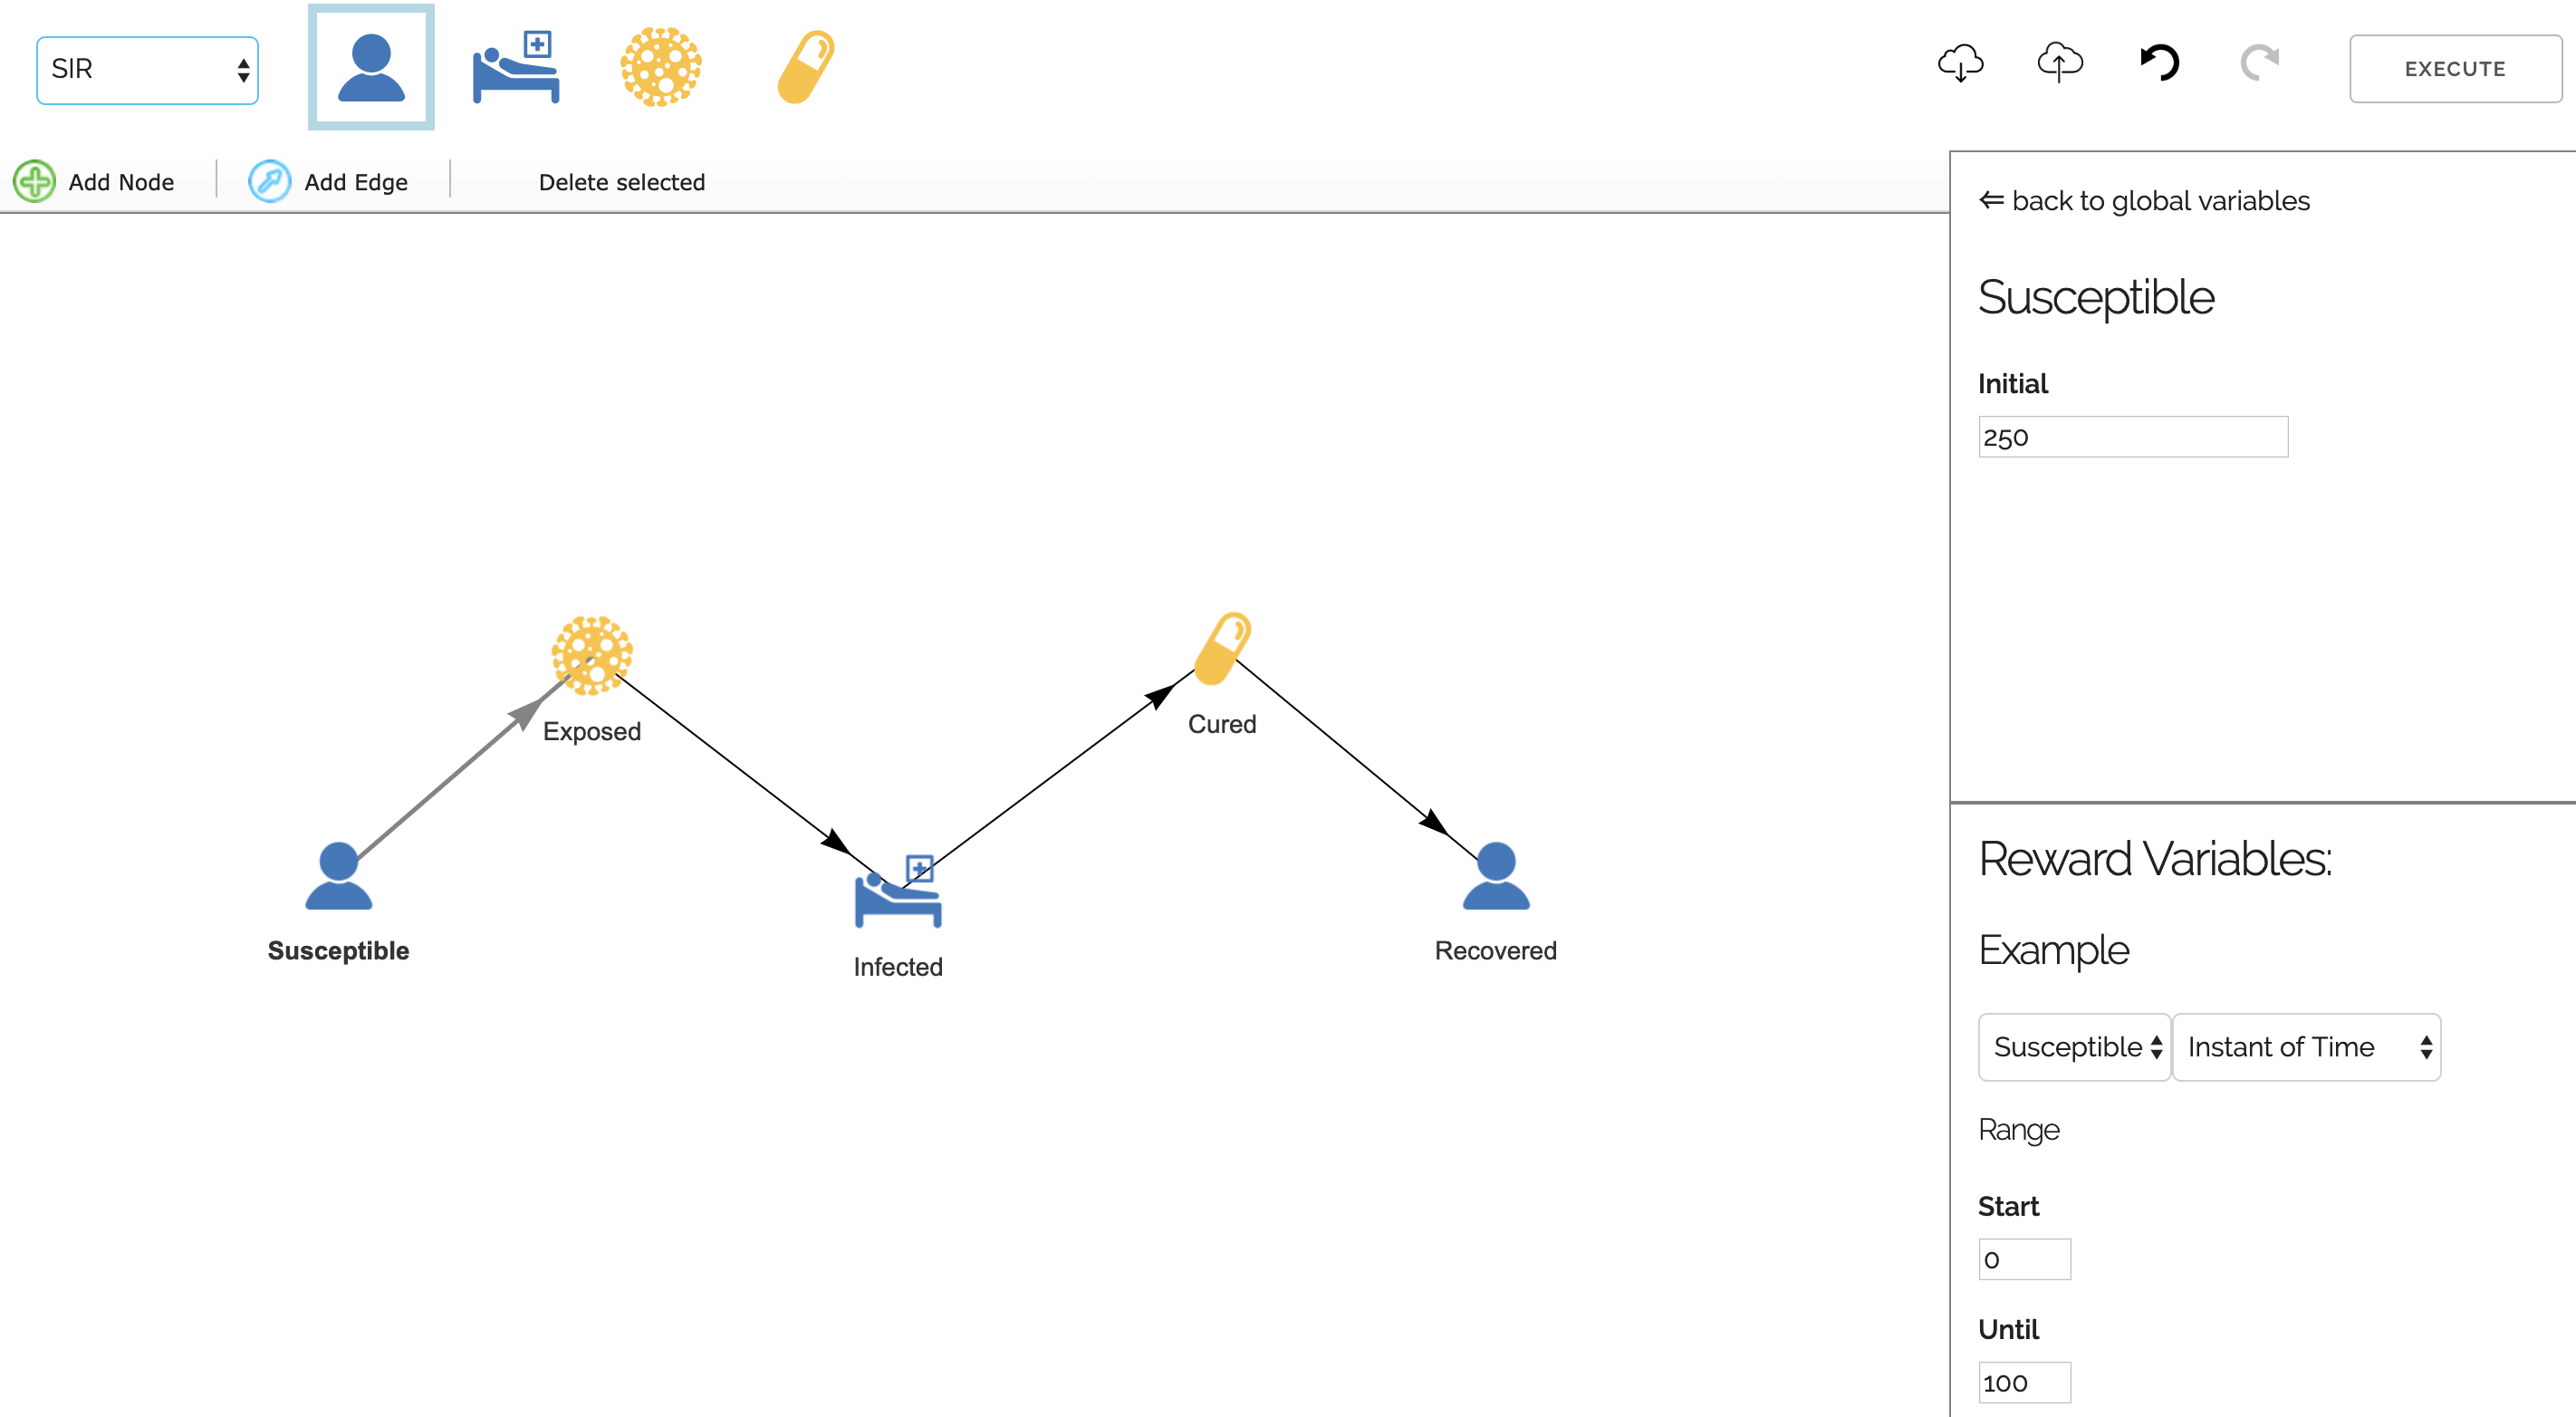
\includegraphics[width=\textwidth]{figs/AMIDOL-UI.png}
\caption{Current Front-End featuring the SIR VDSOL.  The front-end enables the embedding of custom SVGs for nouns and verbs, allowing eventual specialization of produced figures, better matching current domain conventions.}
\label{Fig:Editor}
\end{figure}

\begin{figure}
  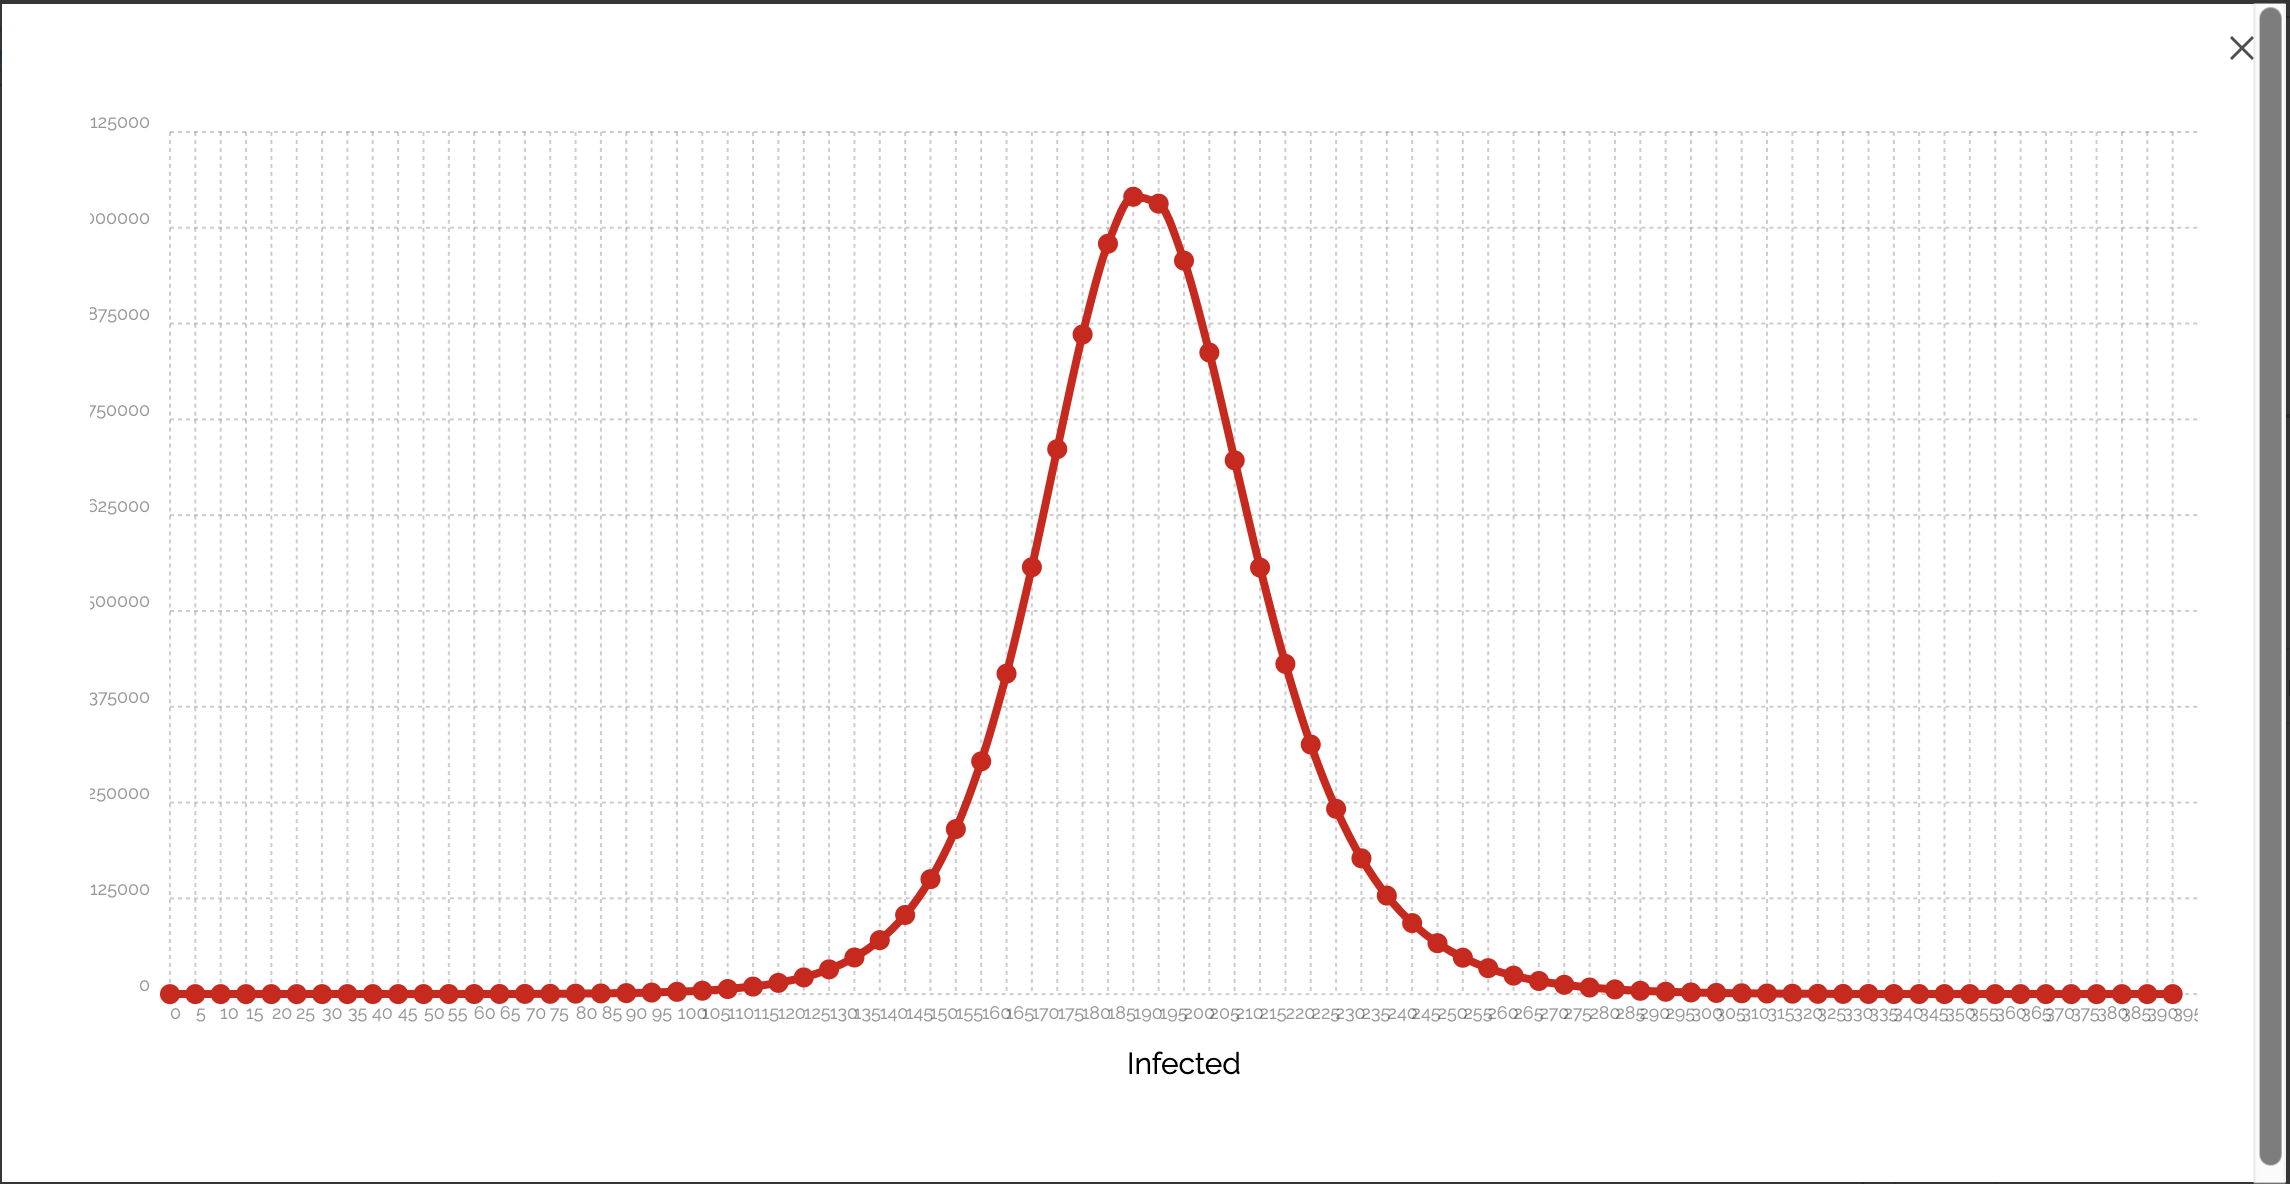
\includegraphics[width=\textwidth]{figs/SIR-output.png}
\caption{Output from the SIR Model in \amidol{}}
\label{Fig:SIROut}
\end{figure}


Figure \ref{Fig:Editor} shows the standard SIR model parameterized to fit real data from the CDC's Influenza B infections for Health and Human Services Region 5 during the 2007-2008 flu season.  Executing this model gives us the results shown in Figure \ref{Fig:SIROut}.

\begin{figure}
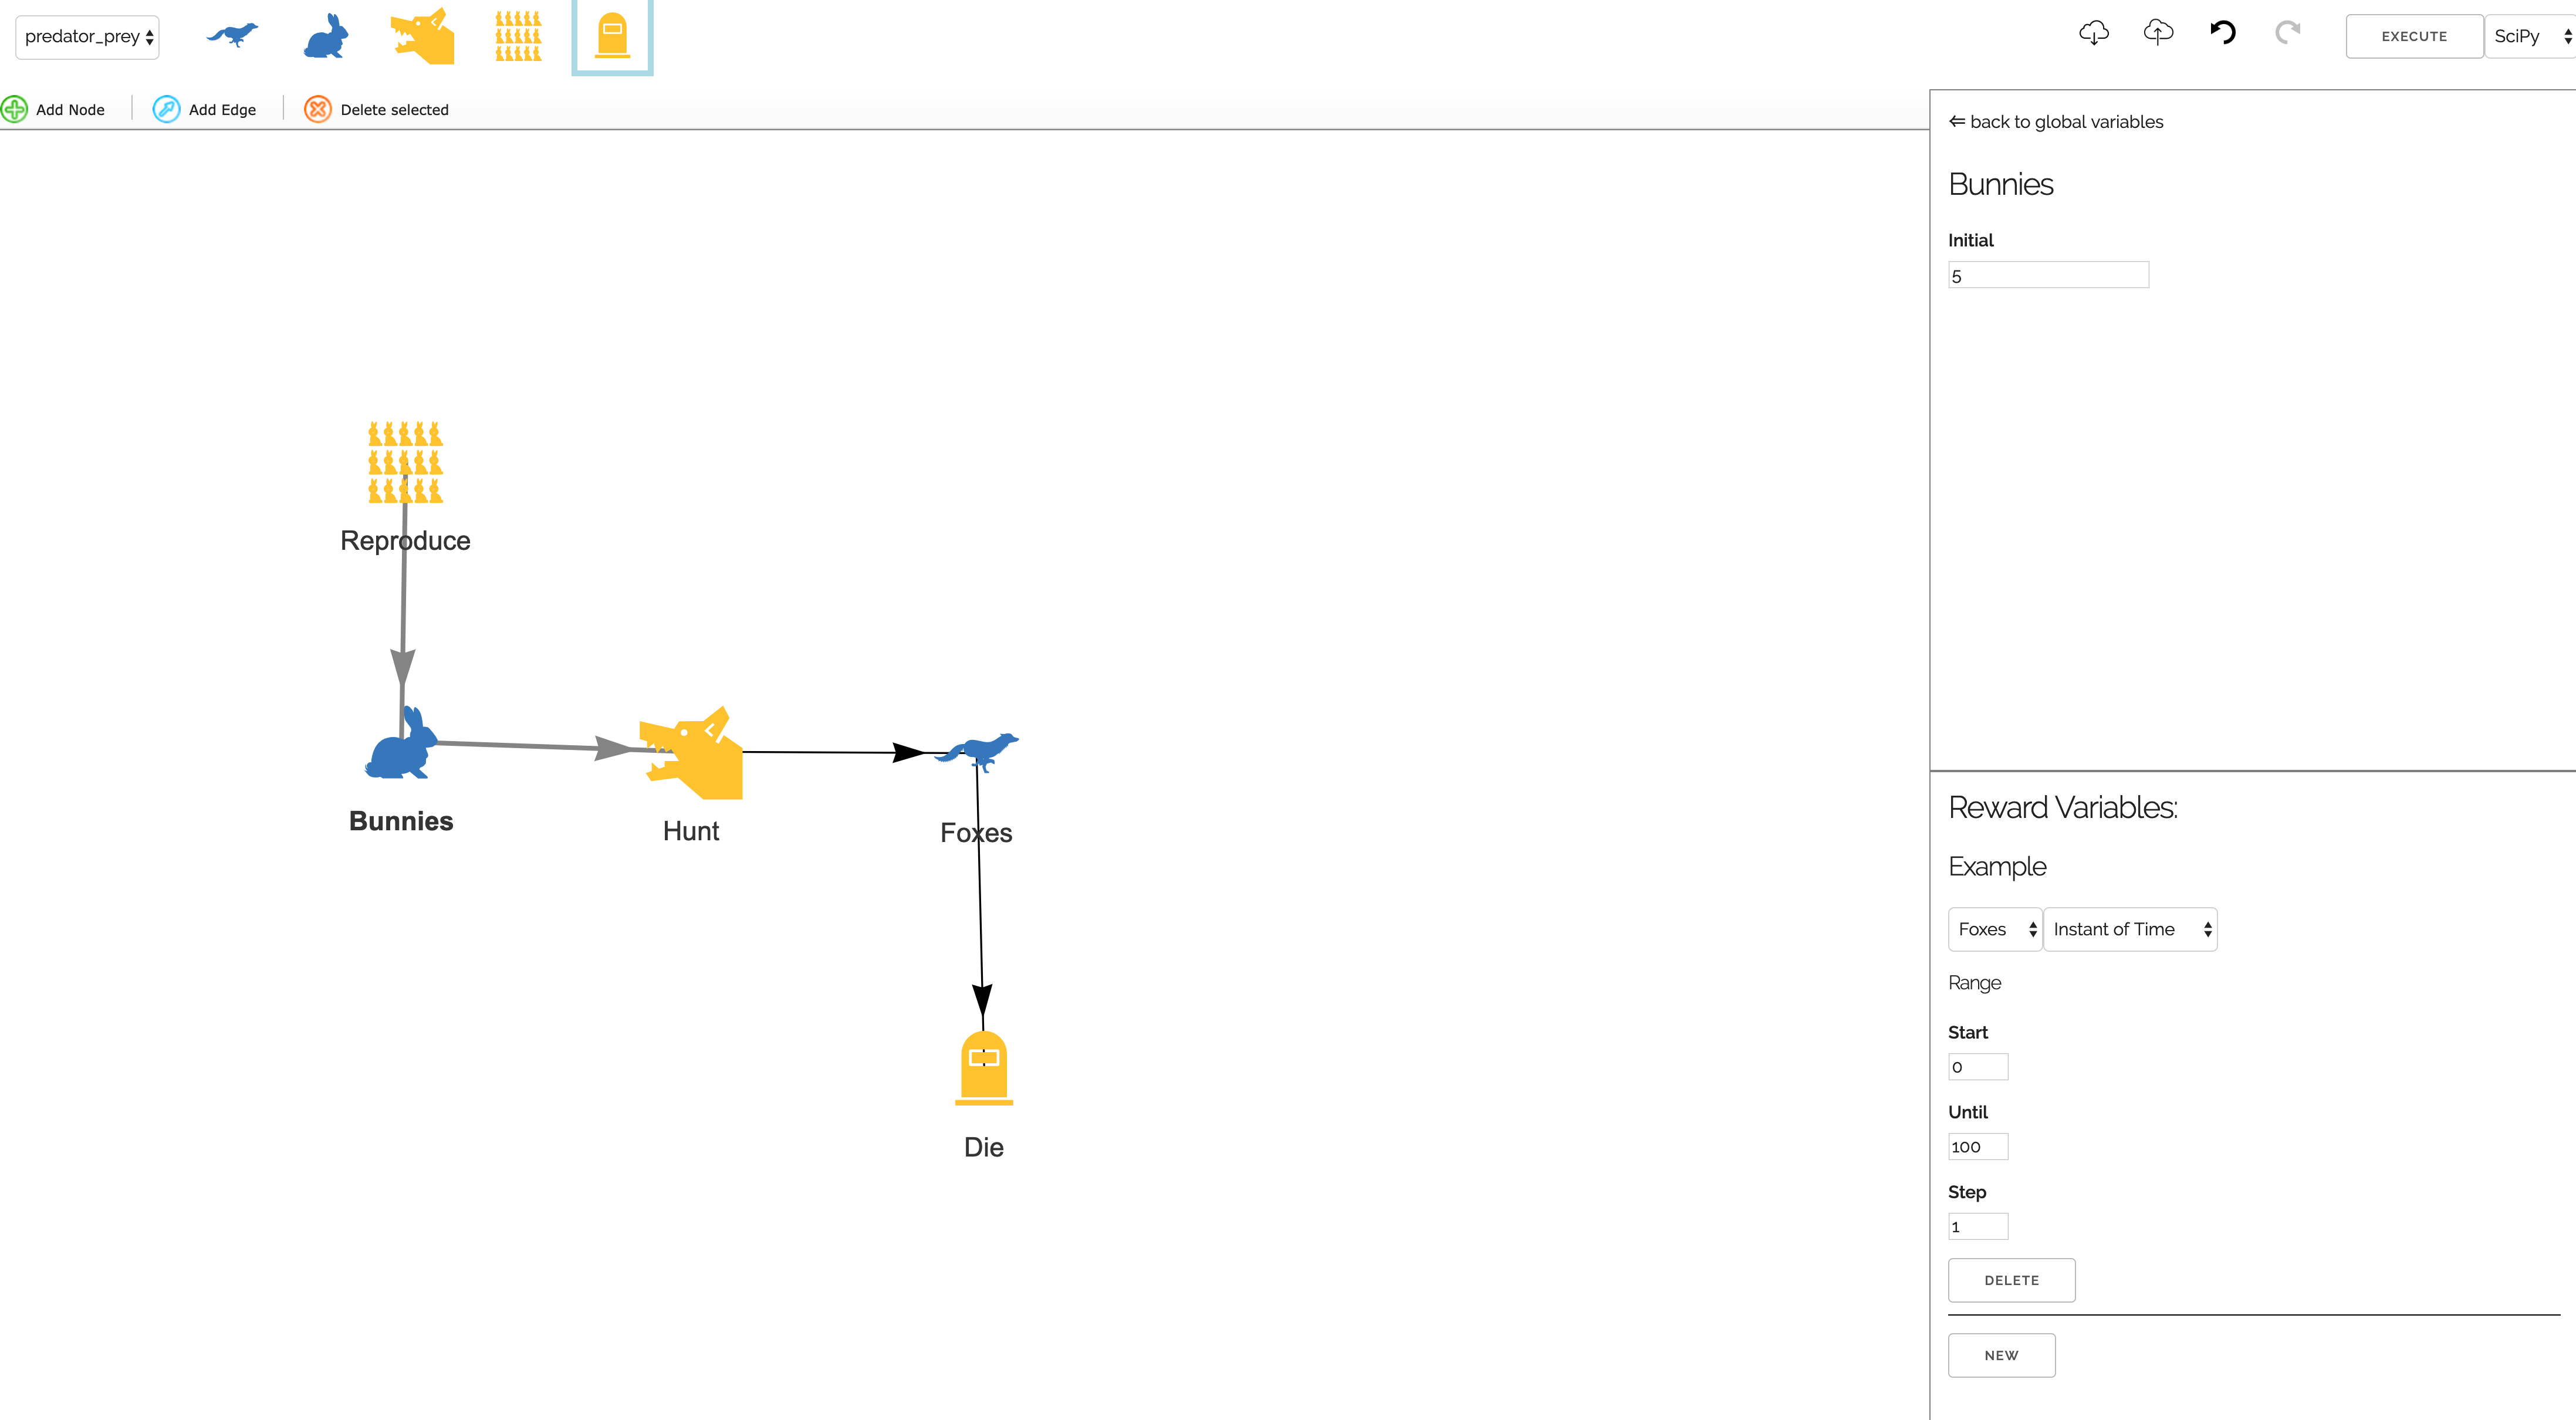
\includegraphics[width=\textwidth]{figs/Lotka-Volterra.png}
\caption{Example Lotka-Volterra Model in \amidol{}.}
\label{Fig:Lotka}
\end{figure}

Figure \ref{Fig:Lotka} shows the Lotka-Volterra model of population dynamics implemented in \amidol{} using the predator-prey palette of nouns and verbs.  This visual diagram is a recreation of semi-formal drawings a domain expert might draw, and meant to be more accessible than the ordinary differential equations which represent this system,

\begin{eqnarray}
  \frac{dx}{dt} &=& \alpha x - \beta x y\\
  \frac{dy}{dt} &=& \delta x y - \gamma y
\end{eqnarray}

Where $x$ is the number of rabbits, and $y$ is the number of foxes.  The \amidol{} translates this drawing automatically into the IR, and from the IR into a SciPy and odeint based representation, resulting in the following executable code:

\begin{lstlisting}[language=python]
  from scipy.integrate import odeint
import json
import numpy as np
import matplotlib.pyplot as plt

class NumpyEncoder(json.JSONEncoder):
    def default(self, obj):
        if isinstance(obj, np.ndarray):
            return obj.tolist()
        return json.JSONEncoder.default(self, obj)

# User defined constants
Example = 0.0

# The ODE system
def deriv_(y_, t_):
    Bunnies, Foxes = y_
    dBunnies_ = 0.0 + 0.66 * Bunnies - 1.0 * Bunnies * Foxes
    dFoxes_ = 0.0 + 4.0 / 3.0 * Bunnies * Foxes - 1.0 * Foxes
    return dBunnies_, dFoxes_

# Boundary conditions and setup
timeRange_ = [ 0.0, 1.0, 2.0, 3.0, 4.0, 5.0, 6.0, 7.0, 8.0, 9.0, 10.0,
11.0, 12.0, 13.0, 14.0, 15.0, 16.0, 17.0, 18.0, 19.0, 20.0, 21.0,
22.0, 23.0, 24.0, 25.0, 26.0, 27.0, 28.0, 29.0, 30.0, 31.0, 32.0,
33.0, 34.0, 35.0, 36.0, 37.0, 38.0, 39.0, 40.0, 41.0, 42.0, 43.0,
44.0, 45.0, 46.0, 47.0, 48.0, 49.0, 50.0, 51.0, 52.0, 53.0, 54.0,
55.0, 56.0, 57.0, 58.0, 59.0, 60.0, 61.0, 62.0, 63.0, 64.0, 65.0,
66.0, 67.0, 68.0, 69.0, 70.0, 71.0, 72.0, 73.0, 74.0, 75.0, 76.0,
77.0, 78.0, 79.0, 80.0, 81.0, 82.0, 83.0, 84.0, 85.0, 86.0, 87.0,
88.0, 89.0, 90.0, 91.0, 92.0, 93.0, 94.0, 95.0, 96.0, 97.0, 98.0,
99.0 ]
y0_ = 5.0, 1.0
output = odeint(deriv_, y0_, timeRange_).T

print(json.dumps(output, cls=NumpyEncoder))
\end{lstlisting}

\begin{figure}
  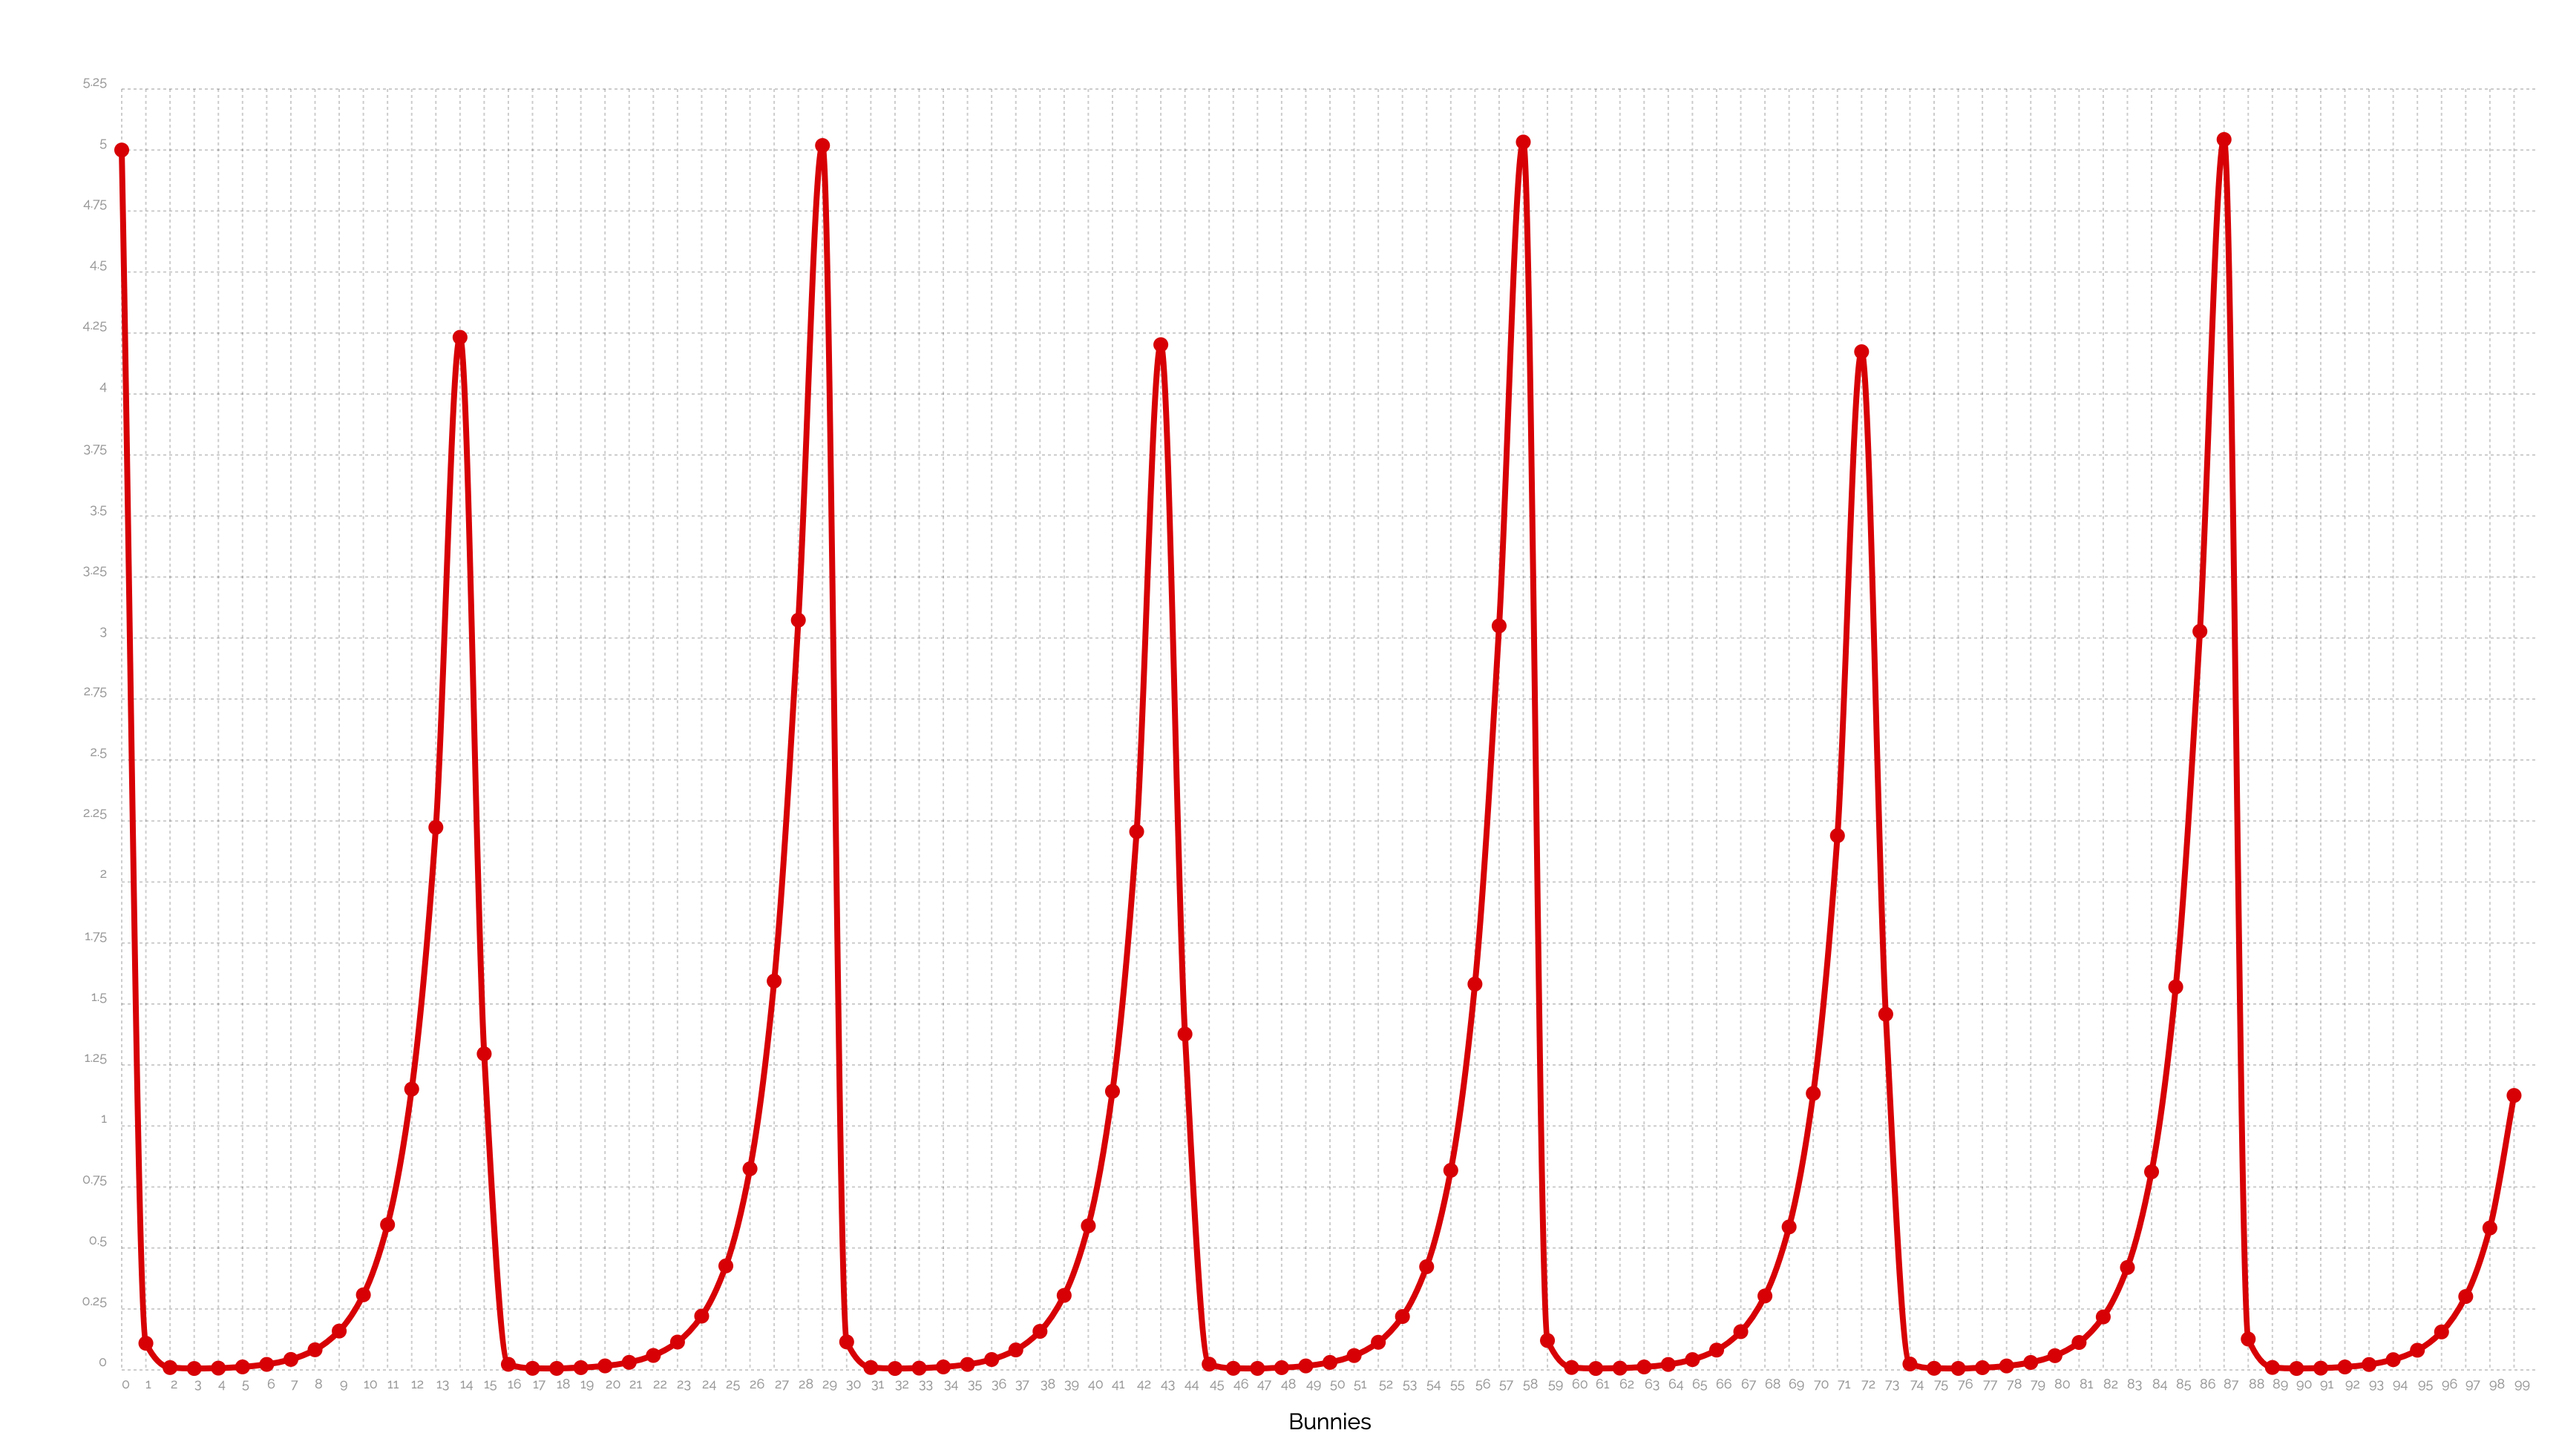
\includegraphics[width=\textwidth]{figs/bunnies.png}
\caption{Output from the Lotka-Volterra in \amidol{}}
\label{Fig:LKOut}
\end{figure}

Figure \ref{Fig:LKOut} shows the current output of the \amidol{} inference engine, matching expectations for the Lotka-Volterra model as parameterized in this example.

\paragraph{A note on the results from the \amidol{} backend}

The Phase 1 prototype currently focuses on a proof of concept for the necessary core technologies of the \amidol{} framework.  During Phase 2 we will be building on the backend's capabilities by implementing a results database and design of experiments interface.  Part of this interface will include extensible plotting and visualization methods given a general form of results.  An early part of our Phase 2 effort will be spent defining a formal results schema and representation, and selecting an appropriate results database to store this schema.  Our design will focus, again, on generalizable techniques that apply to the abstract representations of models, but enable the user to interact with them only through knowledge of the higher level VDSOL concepts.

\subsection{Backend Architecture for IR and Inference Engine}

The backend component interfaces with the UI via a local web server. The idea here is that every time the user interacts with the UI either to modify or to query the model, that information also gets relayed to the backend via a set of web endpoints. When the backend receives new information about the model from the UI, it parses this into some internal representation. This includes such tasks as parsing equations from user-inputted strings and checking that state variables being referred to actually exist. Queries submitted about a model follow a slightly longer path: after being parsed out and validated, the backend figures out how to transform the IR and the query into executable code using reward variables, executes this code, and returns the result back out to the user and eventual results database.

Within the backend, the IR is stored in a graph format resembling what the user constructed in the UI. By maintaining some degree of similarity, we hope to make it simpler to translate results obtained in the backend back out into something end users can easily understand. Queries about models are translated into code artifacts targeting existing solver and simulation programs. We wish to avoid doing actual simulations within the system, instead focusing on intelligently compiling queries into programs that external solvers can run allowing code reuse, and allowing the backend to generate targets for existing, high performance, solver engines. In order to do this we still need to implement a minimum amount of symbolic algebra (e.g. detecting when a continuous rate  model is linear). For the time being, we’ve been targeting Python’s SciPy module as a backend to answer basic simulation questions such as: the the initial value problem for general systems as well as for continuous-time Markov chains.

The backend is written in Scala, leveraging a set of libraries built on top of the Akka actor system for the web server, JSON processing, asynchronous computation, and eventually for the graph in which the IR and data will be stored. The advantages to using Scala include: deployable anywhere the JVM runs, large set of available libraries, and a functional outlook which lends itself well to compiler problems.

\subsection{Integrating AMIDOL}

The JSON API which defines client/server interaction is the only channel by which tangible VDSOL models and the computational AFI/IR communicate. The UI itself doesn't hold any persistent model state which is not represented in a given VDSOL; it is precisely a view or translation of the AFI/IR. This property is what enables the list of integration concepts, and restful architecture.

\section{Next Steps and Phase 2}

The Phase 1 prototype for \amidol{} proves the core technologies and functionality required for success in this project are feasible, achievable, and provide the necessary functionality to support our vision for Phase 2.  Phase 2 will work on extending this base functionality and building on top of our current architecture.  During Phase 2 we will work with more complex models, including full models of H3N2 and H5N1 which include multiple geographic compartments, and the calculation of complex reward variables on these models which require a fully developed Design of Experiments interface as well as model composition.

A large component of our Phase 2 progress will revolve around the use of the results database as a support for tying the results of solving reward variables back to the primitives present in the VDSOL.  A key lesson learned from Phase 1 was the importance of relating reward variables to elements in the VDSOL.  The current state of the art for reward variables involves their definition on model primitives such as state variables and events, which are elements of our IR and not a given VDSOL.  This is not ideal for our goals and desired outcomes which focus on expert interaction with the VDSOL while hiding details of the underlying model.  Our intention is to extend the definition of reward variables in Phase 2 such that we have equivalents for rate and impulse rewards which are instead defined more naturally over nouns and verbs.  We plan to do so by defining reward coupling points in an extension of our VDSOL which indicate what a measure on a noun or a verb will return.  This will allow rewards to be more naturally defined than they currently are both in our prototype and by other modeling tools, and will allow us to infer information on \textbf{structural types} of nouns and verbs, determine equivalences, and capture knowledge from domain experts when they tell us they believe nouns in two different models represent the same abstract quantity.

We intend to collaborate with other performers in the ASKE program, especially TA1 performers, to identify natural ways to import diagrams and models extracted from primary sources, and translate them into \amidol{} models.  This will help show the expressive power of \amidol{}'s system of model definition, and the suitability of the \amidol{} backend and IR as a universal model translation, optimization, and representation layer.

\bibliography{AMIDOL-MWS}

\appendix
\section{Additional Domain Models}

During the course of our work for Phase 1, and in preparation for Phase 2, we have begun identifying and specifying a number of additional models which will help us in our development goals, and in validating our implementations.  Those models are documented in this appendix, but not implemented in our Phase 1 prototype.

\subsection{Artificial Chemistry and Intracellular Viral Infection}

We have also introduced two simple models of artificial chemistry, and viral infection first introduced by \cite{srivastava2002stochastic,haseltine2002approximate} to test different VDSOLs with similar solution techniques.  While simple, models such as the crystallization model:

\begin{eqnarray}
  2A \overset{e_1}{\rightarrow} B\\
  A + C \overset{e_2}{\rightarrow} D
\end{eqnarray}

Allow us to test features of the UI for \amidol{} in a different domain, and the ability of our predicates to handle non-conservation of value in state variables, along with enabling conditions due to the presence of non-renewable reactions.

\begin{figure}
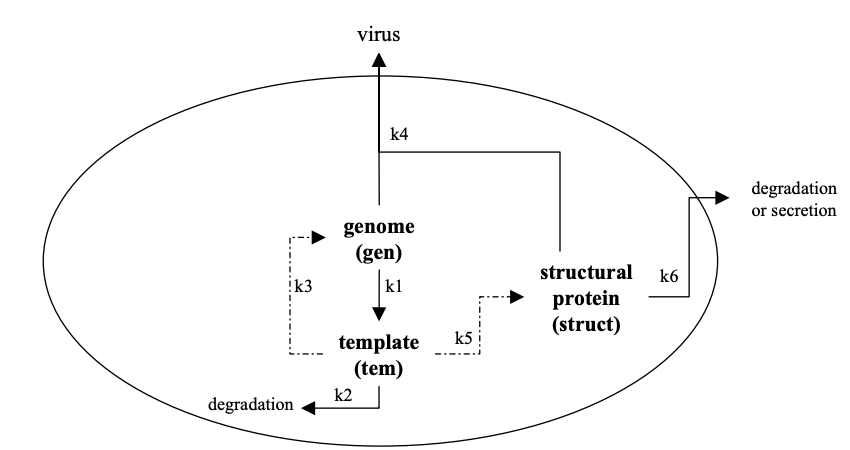
\includegraphics[width=\textwidth]{figs/ViralRep-Crop.png}
\caption{Model of viral replication cycle with catalytic reactions}
\label{Fig:ViralRep}
\end{figure}

Figure \ref{Fig:ViralRep} shows a more complex version of the crystallization model with catalysts, which models viral replication using a chemical kinetic model.

\begin{eqnarray}
\mathrm{nucleotides} \overset{e_1}{\rightarrow} \mathrm{genome}\\
\mathrm{nucleotides} + \mathrm{genome} \overset{e_2}{\rightarrow} \mathrm{template}\\
\mathrm{nucleotides} + \mathrm{aminoacids} \overset{e_3}{\rightarrow} \mathrm{struct}\\
\mathrm{template} \overset{e_4}{\rightarrow} \mathrm{degraded}\\
\mathrm{struct} \overset{e_5}{\rightarrow} \mathrm{secreted}\\
\mathrm{struct} \overset{e_5}{\rightarrow} \mathrm{degraded}\\
\mathrm{genome} + \mathrm{struct} \overset{e_6}{\rightarrow} \mathrm{virus}\\
\end{eqnarray}

This model also features competing events, allowing us to further test our backend's capability for dealing with cases of multiple enabled events.

\subsection{HIV Transactivation Model}

We also employ the HIV Transactivation model presented in \cite{weinberger2005stochastic} as a more complex model of an epidemic process, with the added challenge of handling a system which is stiff, and thus difficult to solve efficiently.  The base model is shown in Figures \ref{Fig:HIV-Tat} and \ref{Fig:HIV-Tat-VDSOL}

\begin{figure}
\begin{subfigure}[b]{\textwidth}
\includegraphics[width=\textwidth]{figs/HIV-Tat-figure.pdf}
\caption{Semi-formal diagram of the molecular model of the Tat transactivation circuit.}
\label{Fig:HIV-Tat}
\end{subfigure}
\begin{subfigure}[b]{\textwidth}
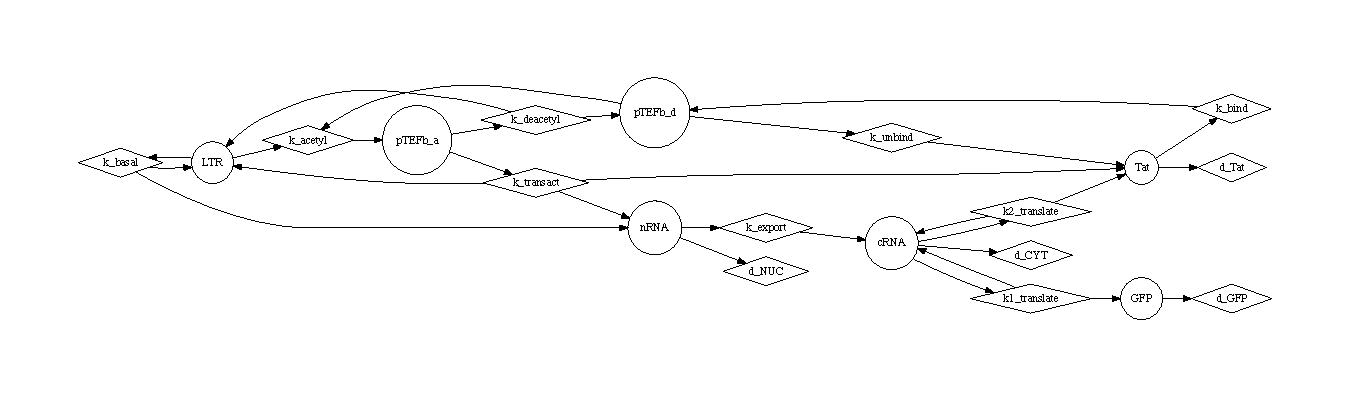
\includegraphics[width=\textwidth]{figs/TatModel.pdf}
\caption{Simple noun (circle) and verb (square) representation of Tat model without ambiguity and aliasing.}
\label{Fig:HIV-Tat-VDSOL}
\end{subfigure}
\end{figure}

Note the use of multiple "Tat" symbols in Figure \ref{Fig:HIV-Tat}. Sometimes scientists draw the same symbol multiple places as an "alias" for the same underlying state variable, which has added the requirement to \amidol{} of supporting entity resolution.  Our goal with \amidol{} is not to fundamentally restrict a domain scientist when drawing diagrams, but rather to assist them in their natural process, and allow them to use the same conventions they are already familiar with, and which exist in their field.

The equations governing this model are given by:

\begin{eqnarray}
LTR \overset{k_{basal}}{\rightarrow} LTR + nRNA\\
nRNA \overset{k_{export}}{\rightarrow} cRNA\\
  cRNA \overset{k1_{translate}}{\rightarrow} GFP + cRNA\\
  cRNA \overset{k2_{translate}}{\rightarrow} Tat + cRNA\\
  Tat \overset{k_{bind}/k_{unbind}}{\leftrightarrow} pTEFb_d\\
  LTR + pTEFb_d \overset{k_{acetyl}/k_{deacetly}}{\leftrightarrow} pTEFb_a\\
  pTEFb_a \overset{k_{transact}}{\leftrightarrow} LTR + nRNA + Tat\\
  GFP \overset{d_{GFP}}{\rightarrow} \emptyset\\
  Tat \overset{d_{Tat}}{\rightarrow} \emptyset\\
  cRNA \overset{d_{CYT}}{\rightarrow} \emptyset\\
  nRNA \overset{d_{NUC}}{\rightarrow} \emptyset
\end{eqnarray}

Using real data generated with flow cytometry, this model can be parameterized as follows:

\begin{eqnarray}
k_basal &=& 10^{-8} (transcripts/s)\\
  k_export &=& 0.00072 (1/s)\\
  k1_translate &=& 0.5 (1/s)\\
  k2_translate &=& 0.005 (1/s)\\
  k_bind &=& 10^{-4} (1/(mol * s))\\
  k_unbind &=& 10^{-2} (1/s)\\
  k_acetyl &=& 10^{-3} (1/(mol * s))\\
  k_deacetyl &=& 0.9 (1/s)\\
  k_transact &=& 0.1 (1/s)
\end{eqnarray}

As can be seen, the rates differ by many orders of magnitude, a situation that causes the model to be classified as stiff, and thus difficult to solve by many ODE techniques.  We are using this model to test the Design of Experiments capability of \amidol{} to automatically select appropriate solution techniques for a user, avoiding numerical instability and the use of inefficient algorithms which otherwise could be pitfalls for traditional modeling methods.


\end{document}

%  LocalWords:  textbf Composability lampka2002symbolic mathbb ldots
%  LocalWords:  sanders1992dependability,sanders1988construction cdot
%  LocalWords:  sanders1995ultrasan rightarrow infty mathcal cdot t,t
%  LocalWords:  qureshi1996algorithms,deavours1999efficient,ciardo1996well
%  LocalWords:  freire1990technique t,t includegraphics textwidth
%  LocalWords:  Plackett-Burman Fluview cdc2019fluview eqnarray
%  LocalWords:  bailis2005mortality,murphy2004quantification mathrm
%  LocalWords:  morris1991factorial fraser2009pandemic mathrm texttt
%  LocalWords:  fisman2014early aminoacids weinberger2005stochastic
%  LocalWords:  srivastava2002stochastic,haseltine2002approximate
%  LocalWords:  deacetly emptyset cytometry k_deacetyl texttt
